%definira klasu dokumenta 
\documentclass[12pt]{report} 

%prostor izmedu naredbi \documentclass i \begin{document} se zove uvod. U njemu se nalaze naredbe koje se odnose na cijeli dokument

%osnovni LaTex ne može riješiti sve probleme, pa se koriste različiti paketi koji olakšavaju izradu željenog dokumenta
\usepackage[croatian]{babel} 
\usepackage{amssymb}
\usepackage{amsmath}
\usepackage{txfonts}
\usepackage{mathdots}
\usepackage{titlesec}
\usepackage{array}
\usepackage{lastpage}
\usepackage{etoolbox}
\usepackage{longtable, tabu}
\usepackage{color, colortbl}
\usepackage{adjustbox}
\usepackage{geometry}
\usepackage[classicReIm]{kpfonts}
\usepackage{hyperref}
\usepackage{fancyhdr}

\usepackage{float}
\usepackage{setspace}
\restylefloat{table}
\usepackage{enumitem}
\usepackage{listings}
\usepackage{color}

\definecolor{dkgreen}{rgb}{0,0.6,0}
\definecolor{gray}{rgb}{0.5,0.5,0.5}
\definecolor{mauve}{rgb}{0.58,0,0.82}

\lstset{frame=tb,
	language=Java,
	aboveskip=3mm,
	belowskip=3mm,
	showstringspaces=false,
	columns=flexible,
	basicstyle={\small\ttfamily},
	numbers=none,
	numberstyle=\tiny\color{gray},
	keywordstyle=\color{blue},
	commentstyle=\color{dkgreen},
	stringstyle=\color{mauve},
	breaklines=true,
	breakatwhitespace=true,
	tabsize=1
}


\patchcmd{\chapter}{\thispagestyle{plain}}{\thispagestyle{fancy}}{}{} %redefiniranje stila stranice u paketu fancyhdr

%oblik naslova poglavlja
\titleformat{\chapter}{\normalfont\huge\bfseries}{\thechapter.}{20pt}{\Huge}
\titlespacing{\chapter}{0pt}{0pt}{40pt}


\linespread{1.3} %razmak između redaka

\geometry{a4paper, left=1in, top=1in,}  %oblik stranice

\hypersetup{ colorlinks, citecolor=black, filecolor=black, linkcolor=black,	urlcolor=black }   %izgled poveznice


%prored smanjen između redaka u nabrajanjima i popisima
\newenvironment{packed_enum}{
	\begin{enumerate}
		\setlength{\itemsep}{0pt}
		\setlength{\parskip}{0pt}
		\setlength{\parsep}{0pt}
	}{\end{enumerate}}

\newenvironment{packed_item}{
	\begin{itemize}
		\setlength{\itemsep}{0pt}
		\setlength{\parskip}{0pt}
		\setlength{\parsep}{0pt}
	}{\end{itemize}}


%boja za privatni i udaljeni kljuc u tablicama
\definecolor{LightBlue}{rgb}{0.9,0.9,1}
\definecolor{LightGreen}{rgb}{0.9,1,0.9}


%podesavanje zaglavlja i podnožja

\pagestyle{fancy}
\lhead{Programsko inženjerstvo}
\rhead{Planinarski dnevnik}
\lfoot{RuntimeTerror}
\cfoot{stranica \thepage/\pageref{LastPage}}
\rfoot{\today}
\renewcommand{\headrulewidth}{0.2pt}
\renewcommand{\footrulewidth}{0.2pt}


\begin{document} 
	
	
	
	\begin{titlepage}
		\begin{center}
			\vspace*{\stretch{1.0}} %u kombinaciji s ostalim \vspace naredbama definira razmak između redaka teksta
			\LARGE Programsko inženjerstvo\\
			\large Ak. god. 2020./2021.\\
			
			\vspace*{\stretch{3.0}}
			
			\huge{Planinarski Dnevnik}\\
			\Large Dokumentacija, Rev. \textit{$1.6$}\\
			
			\vspace*{\stretch{12.0}}
			\normalsize
			Grupa: \textit{$RuntimeTerror$}\\
			Voditelj: \textit{Ivan Martinović}\\
			
			
			\vspace*{\stretch{1.0}}
			Datum predaje: \textit{13.11.2020.}\\
	
			\vspace*{\stretch{4.0}}
			
			Nastavnik: \textit{Katarina Labor}\\
		
		\end{center}

	
	\end{titlepage}

	
	\tableofcontents

	\chapter{Dnevnik promjena dokumentacije}
		
		%\textbf{\textit{Kontinuirano osvježavanje}}\\
				
		
		\begin{longtabu} to \textwidth {|X[2, l]|X[13, l]|X[3, l]|X[3, l]|}
			\hline \multicolumn{1}{|l|}{\textbf{Rev.}}	& \multicolumn{1}{l|}{\textbf{Opis promjene/dodatka}} & \multicolumn{1}{|l|}{\textbf{Autori}} & \multicolumn{1}{l|}{\textbf{Datum}} \\[3pt] \hline
			\endfirsthead
			
			\hline \multicolumn{1}{|l|}{\textbf{Rev.}}	& \multicolumn{1}{l|}{\textbf{Opis promjene/dodatka}} & \multicolumn{1}{|l|}{\textbf{Autori}} & \multicolumn{1}{l|}{\textbf{Datum}} \\[3pt] \hline
			\endhead
			
			\hline 
			\endlastfoot
			
			0.1 & Napravljen predložak.	& I.M & 14.10.2020. 		\\[3pt] \hline 
			0.2	& Dodan opis projektnog zadatka & J.K, H.L, N.K, I.M, D.K & 14.10.2020. 	\\[3pt] \hline 
			0.3 & Dodana osnovna verzija funkcionalnih zahtjeva & J.K, I.M, M.R & 14.10.2020. \\[3pt] \hline 
			0.3.1 & Ispravljeni funkcionalni zahtjevi & I.M & 17.10.2020 \\[3pt] \hline 
			0.4 & Dodana početna verzija obrazaca uporabe & D.K, N.K & 19.10.2020 \\[3pt] \hline 
			0.4.1 & Ispravljeni, povezani i dodani novi scenariji obrazaca uporabe  & I.M & 21.10.2020. \\[3pt] \hline 
			0.4.2 & Izmijenjeni i dodani novi obrasci uporabe & I.M & 25.10.2020 \\[3pt] \hline 
			0.5 & Dodani dijagrami obrazaca uporabe & I.M & 25.10.2020 \\[3pt] \hline 
			0.6 & Dodani sekvencijski dijagrami & J.K, H.L, I.M & 29.10.2020 \\[3pt] \hline 
			0.7 & Dodan opis baze podataka zajedno s tablicama & M.R, I.M & 05.11.2020 \\[3pt] \hline 
			0.7.1 & Dodani nefunkcionalni zahtjevi te zahtjevi domene primjene & D.K, N.K & 05.11.2020 \\[3pt] \hline 
			0.8 & Dodan opis arhitekture sustava & J.K & 5.11.2020 \\[3pt] \hline 
			0.8.1 & Ažuriran opis baze podataka, preimenovane tablice i dorađeni atributi & I.M & 10.11.2020 \\[3pt] \hline
			%1.2 & Manje izmjene:Timer - Brojilo vremena & Grudenić & 15.09.2013. \\[3pt] \hline 
			%1.3 & Popravljeni dijagrami obrazaca uporabe & Jović & 15.09.2013. \\[3pt] \hline 
			%1.5 & Generalna revizija strukture dokumenta & Ivošević & 19.09.2013. \\[3pt] \hline 
			%1.5.1 & Manja revizija (dijagram razmještaja) & Jović & 20.09.2013. \\[3pt] \hline 
			%\textbf{2.0} & Konačni tekst predloška dokumentacije  & Ivošević & 28.09.2013. \\[3pt] \hline 
			%&  &  & \\[3pt] \hline
			
			
		\end{longtabu}
	
	\chapter{Opis projektnog zadatka}
		
		%\textbf{\textit{dio 1. revizije}}\\
		
		U današnje vrijeme većina ljudi živi užurbanim tempom, stoga svaki slobodan trenutak žele iskoristiti za odmor i rekreaciju. Mnoge ljude privlači boravak na svježem zraku te kao rezultat toga, sve više ljudi izabire planinarenje kao jednu od brojnih mogućnosti koje im se nude. Međutim, planinari pri odabiru rute za svoje planinarske izlete često nemaju dovoljno informacija pa se koriste usmenom predajom i nagađanjima. Tako planinari, osobito planinari rekreativci, nailaze na različite probleme od kojih su najčešći krive informacije o stazama i rutama ili planinarski domovi bez odgovarajuće infrastrukture. Upravo zbog toga pokrenut je projekt čiji je cilj razvoj i evolucija programskog proizvoda, odnosno web aplikacije „Planinarski dnevnik“. Aplikacija će uvelike pomoći planinarima u organiziranju svojih planinarskih izleta, ali i ponuditi točne informacije o rutama na pojedinim izletima te povezati planinare poznanike u vlastitu planinarsku zajednicu. Osim toga, planinari će moći pretraživati i planinarske domove koji se nalaze na odabranim stazama, a za svaki dom će biti prikazane koje pogodnosti on nudi (prenoćište, topao obrok, pitka voda, struja, grijanje itd.). \\
		
		Opseg projektnog zadatka sadrži sve aktivnosti i zadatke koji su vezani uz izradu aplikacije. Za početak se radi analiza aplikacije kako bi se utvrdilo koliko će okvirno vremena biti potrebno za izradu određene komponente aplikacije. U tome dobrim dijelom pomažu dnevnik sastajanja i dnevnik aktivnosti koji služe kao kontrolne točke pomoću kojih se vidi ide li daljnji napredak aplikacije u dobrom smjeru. Na tim sastancima prisutni su asistenti koji su stručnjaci za ovo područje i svojim savjetima višestruko pomažu timu. \\
		
		Za izradu „Planinarskog dnevnika“ predviđen je vremenski period od 13 tjedana, odnosno jednog fakultetskog semestra. Radi se analiza interesnih sudionika s namjerom da se što točnije odredi broj korisnika koji će biti zainteresirani za korištenje aplikacije. Svrha same aplikacije je educirati studente na fakultetu pa shodno tome ne postoje troškovi prilikom izrade iste. Krajnji cilj je potpuno razvijena aplikacija s ispravnom programskom potporom koja sadrži sve zahtijevane komponente i podržava rad više korisnika u stvarnom vremenu. Kada je navedeno postignuto, aplikacija je spremna za lansiranje na tržište kako bi se korisnici mogli njome služiti.\\
		
		Aplikacija „Planinarski dnevnik“ zasigurno će biti najzanimljivija planinarima kojima je i namijenjena, ali također i mnogobrojnim ustanovama poput planinarskih domova kojima će omogućiti promociju u širem krugu korisnika. Potencijalno bi moglo doći do povećanja prihoda kao rezultat brojnih usluga koje planinarski domovi pružaju, ali i poboljšanja kvalitete istih sukladno s porastom broja planinara koji ih posjećuju. Proširit će se opseg planinarskog turizma na manje poznata područja tako što će postati vidljiva širem krugu korisnika aplikacije. Također, korisnost ove aplikacije odrazit će se na HGSS (Hrvatska gorska služba spašavanja) koja će efikasnije saznati sve potrebne informacije o kretanju i ruti planinara u slučaju nesreće ili nestanka. Evidentno je da će se područje pretrage znatno smanjiti jer će planinar unaprijed odrediti rutu svojeg kretanja.\\
		
		Pokretanjem aplikacije svakom korisniku prvotno će biti dodijeljena uloga \underbar{Gost} koja omogućava pretraživanje postojećih planinarskih domova prema dostupnoj infrastrukturi (pitka voda, hrana, prenoćište...) ili
		pretraživanje planinarskih staza prema zahtjevnosti, trajanju ili duljini. Za sve daljnje aktivnosti korisnik će se morati registrirati u sustav tako što će u predloženu formu za registraciju unijeti osobne podatke:
		\begin{packed_item}
			\item ime
			\item prezime
			\item e-mail
			\item lozinku
			\item sliku (opcionalno)
			\item nešto više o sebi (opcionalno)
			\item datum rođenja (opcionalno)
			\item mjesto stanovanja (opcionalno)	
		\end{packed_item}
	 
		Nakon što se korisnik registrira dodijelit će mu se uloga \underbar{Planinar} i moći će pristupiti vlastitom profilu. Omogućit će mu se pregled i uređivanje osobnih podataka te u krajnjem slučaju uklanjanje korisničkog računa. Planinar može uspostaviti odnos s ostalim registriranim planinarima tako što šalje zahtjeve za "prijateljstvom", odnosno zahtjeve za dodavanje na popis vlastite planinarske zajednice, ali i na način da ostale članove svoje planinarske zajednice pozove na određeni događaj. Prema unaprijed određenom predlošku dopušta se stvaranje vlastitih planinarskih staza kao i vlastitih događaja. Uz to se nudi i mogućnost ocjenjivanja stvorenih planinarskih staza kao i prijava netočnih ili nepreciznih informacija vezanih uz pojedine staze, što može biti od velike koristi svim planinarima, osobito početnicima koji na osnovu najviše ocjene mogu odabrati svoju željenu stazu. Na naslovnici će biti prikazane objave prijatelja planinara, a na zidu obavijesti će biti vidljiv popis prihvaćenih ili odbijenih pozivnica te prihvaćenih ili odbijenih zahtjeva za prijateljstvom. Nudi se i svrstavanje planinarske staze ili doma na popis željenih te dodavanje ranije odrađenih planinarskih staza u osobnu arhivu. Dolaskom planinara na cilj evidentirat će se njihovo prisutstvo, a nakon određenog broja osvojenih vrhova ostvarit će pravo na bedž kao jednu vrstu motivacije za još veću aktivnost u budućnosti. \\
		
		Sustav nadgleda \underbar{Administrator} koji ima najveće ovlasti. Ukoliko neki korisnik (planinar) ne poštuje pravila ponašanja, administrator ima pravo obrisati njegov korisnički račun. On će zaprimati primjedbe od korisnika na određene staze te će ovisno o količini netočnih informacija odlučiti hoće li staza biti izmijenjena ili uklonjena s liste. Time se sprječava ponavljanje istih pogrešaka u budućnosti i aplikacija će biti sve točnija i vjerodostojnija. 
		
		
		\section{Primjeri sličnih rješenja}
		Slične implementacije rješenja projektnog zadatka već postoje. Na području Republike Hrvatske možemo izdvojiti iduće: 
		\begin{packed_enum}
			\item Kao prvi primjer navodimo aplikaciju \textbf{eHPS} koja je razvijena pod pokroviteljstvom Hrvatskog planinarskog saveza. Njena svrha je omogućavanje korisniku efikasno pretraživanje podataka o svim planinarskim domovima, kućama i skloništima koji postoje na području Republike Hrvatske. Također pruža uslugu iščitavanja i proučavanja podataka o svim kontrolnim točkama i dosad otvorenim planinarskim obilaznicama.
			\item Druga slična aplikacija je \textbf{infoHPS} koja pruža uslugu pretraživanja postojećih planinarskih udruga koje su članice Hrvatskog planinarskog saveza. Za svaku traženu udrugu omogućuje prikaz informacija bitnih za korisnika poput naziva, OIB-a udruge, email-a itd. 
		\end{packed_enum}
	
			\begin{figure}[H]
			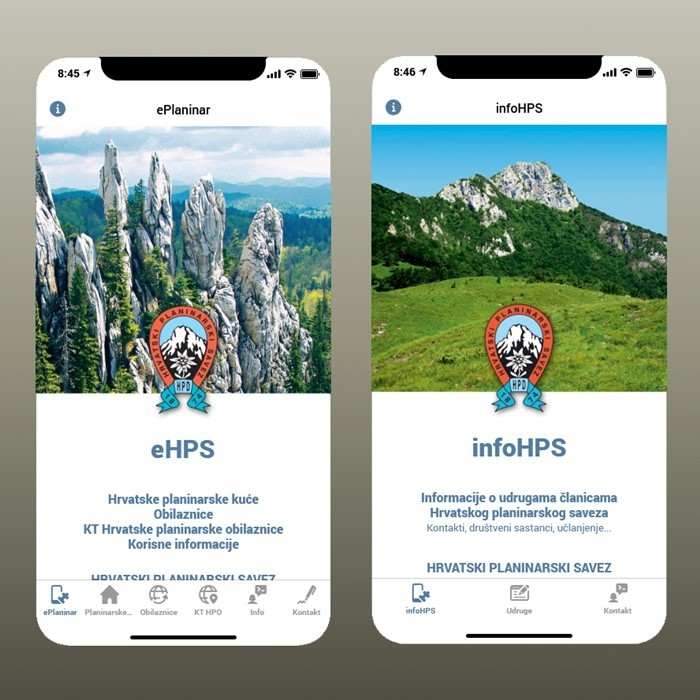
\includegraphics[scale=0.5]{slike/HPS.jpg} %veličina slike u odnosu na originalnu datoteku i pozicija slike
			\centering
			\caption{Primjeri sličnih aplikacija - eHPS i infoHPS}
			\label{fig:slične aplikacije}
			\end{figure}
	
		Na području SAD-a aplikacija \textbf{Mountain project} nudi korisnicima pretraživanje postojećih planinarskih ruta, čitanje novosti i razmjenjivanje poruka između prijavljenih korisnika.
			
			\begin{figure}[H]
				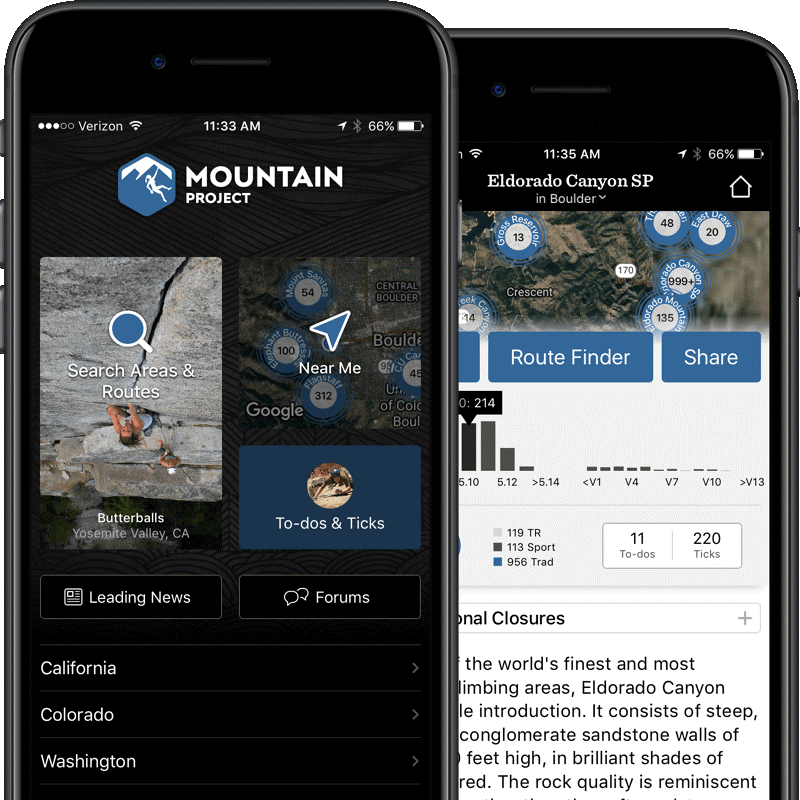
\includegraphics[scale=0.3]{slike/mountainproject.png} %veličina slike u odnosu na originalnu datoteku i pozicija slike
				\centering
				\caption{Primjer slične aplikacije - Mountain Project}
				\label{fig:slične aplikacije}
			\end{figure}
		
		\section{Moguće nadogradnje projektnog zadatka}
		Postoje brojne funkcionalnosti kojima bi se mogla nadograditi i proširiti postojeća aplikacija te ispraviti eventualne nepravilnosti. Jedna od mogućnosti je implementacija „Chat-a“ za razmjenu poruka i iskustava među planinarima koji pripadaju istoj planinarskoj zajednici. Uz to, mogao bi se dodati i neformalni forum gdje bi svi planinari mogli podijeliti svoja iskustva, doživljaje i preporuke ostatku planinarske zajednice. Aplikacija bi trebala imati i mogućnost instaliranja na pametne satove koji su postali neizostavni dio planinarske i sportske opreme.  Također bi bilo korisno kad bi korisnici odlaskom na naslovnu stranu aplikacije mogli vidjeti aktualne novosti, događanja iz planinarskog svijeta te preporučene izlete u skladu s vremenskim uvjetima. Svaki planinar mora imati odgovarajuću opremu prije nego što krene na izlet pa bi oglašavanje i prodaja planinarske opreme bio izvrstan dodatak aplikaciji. Registrirani planinar bi mogao postaviti oglas sa slikom i opisom opreme koju prodaje, cijenom i lokacijom na kojoj se nalazi. Sadašnja verzija aplikacije sadrži unesene izlete namijenjene većinom za pješačke rute. U budućnosti bi se aplikacija mogla proširiti dodavanjem ruta za bicikliranje ili čak i skijanje. Još jedna od korisnih funkcionalnosti bila bi uvođenje uloge „planinarski dom“. Uloga bi planinarskim domovima omogućila kreiranje vlastitih događaja kao što su organizirani izleti, zabave i slično. 
		
		\eject
		
	
	\chapter{Specifikacija programske potpore}
		
	\section{Funkcionalni zahtjevi}
			
			\textbf{\textit{dio 1. revizije}}\\
			
			\textit{Navesti \textbf{dionike} koji imaju \textbf{interes u ovom sustavu} ili  \textbf{su nositelji odgovornosti}. To su prije svega korisnici, ali i administratori sustava, naručitelji, razvojni tim.}\\
				
			\textit{Navesti \textbf{aktore} koji izravno \textbf{koriste} ili \textbf{komuniciraju sa sustavom}. Oni mogu imati inicijatorsku ulogu, tj. započinju određene procese u sustavu ili samo sudioničku ulogu, tj. obavljaju određeni posao. Za svakog aktora navesti funkcionalne zahtjeve koji se na njega odnose.}\\
			
			
			\noindent \textbf{Dionici:}
			
			\begin{packed_enum}
				
				\item Dionik 1
				\item Dionik 2				
				\item ...
				
			\end{packed_enum}
			
			\noindent \textbf{Aktori i njihovi funkcionalni zahtjevi:}
			
			
			\begin{packed_enum}
				\item  \underbar{Aktor 1 (inicijator) može:}
				
				\begin{packed_enum}
					
					\item funkcionalnost 1
					\item funkcionalnost 2
					\begin{packed_enum}
						
						\item  podfunkcionalnost 1 
						\item  podfunkcionalnost 2
				
					\end{packed_enum}
					\item  funkcionalnost 3
					
				\end{packed_enum}
			
				\item  \underbar{Aktor 2 (sudionik) može:}
				
				\begin{packed_enum}
					
					\item funkcionalnost 1
					\item funkcionalnost 2
					
				\end{packed_enum}
			\end{packed_enum}
			
			\eject 
			
			
				
			\subsection{Obrasci uporabe}
				
				\textbf{\textit{dio 1. revizije}}
				
				\subsubsection{Opis obrazaca uporabe}
					\textit{Funkcionalne zahtjeve razraditi u obliku obrazaca uporabe. Svaki obrazac je potrebno razraditi prema donjem predlošku. Ukoliko u nekom koraku može doći do odstupanja, potrebno je to odstupanje opisati i po mogućnosti ponuditi rješenje kojim bi se tijek obrasca vratio na osnovni tijek.}\\
					

					\noindent \underbar{\textbf{UC$<$broj obrasca$>$ -$<$ime obrasca$>$}}
					\begin{packed_item}
	
						\item \textbf{Glavni sudionik: }$<$sudionik$>$
						\item  \textbf{Cilj:} $<$cilj$>$
						\item  \textbf{Sudionici:} $<$sudionici$>$
						\item  \textbf{Preduvjet:} $<$preduvjet$>$
						\item  \textbf{Opis osnovnog tijeka:}
						
						\item[] \begin{packed_enum}
	
							\item $<$opis korak jedan$>$
							\item $<$opis korak dva$>$
							\item $<$opis korak tri$>$
							\item $<$opis korak četiri$>$
							\item $<$opis korak pet$>$
						\end{packed_enum}
						
						\item  \textbf{Opis mogućih odstupanja:}
						
						\item[] \begin{packed_item}
	
							\item[2.a] $<$opis mogućeg scenarija odstupanja u koraku 2$>$
							\item[] \begin{packed_enum}
								
								\item $<$opis rješenja mogućeg scenarija korak 1$>$
								\item $<$opis rješenja mogućeg scenarija korak 2$>$
								
							\end{packed_enum}
							\item[2.b] $<$opis mogućeg scenarija odstupanja u koraku 2$>$
							\item[3.a] $<$opis mogućeg scenarija odstupanja  u koraku 3$>$
							
						\end{packed_item}
					\end{packed_item}
				
					
				\subsubsection{Dijagrami obrazaca uporabe}
					
					\textit{Prikazati odnos aktora i obrazaca uporabe odgovarajućim UML dijagramom. Nije nužno nacrtati sve na jednom dijagramu. Modelirati po razinama apstrakcije i skupovima srodnih funkcionalnosti.}
				\eject		
				
			\subsection{Sekvencijski dijagrami}
				
				\textbf{\textit{dio 1. revizije}}\\
				
				\textit{Nacrtati sekvencijske dijagrame koji modeliraju najvažnije dijelove sustava (max. 4 dijagrama). Ukoliko postoji nedoumica oko odabira, razjasniti s asistentom. Uz svaki dijagram napisati detaljni opis dijagrama.}
				\eject
	
		\section{Ostali zahtjevi}
		
			\textbf{\textit{dio 1. revizije}}\\
		 
			 \textit{Nefunkcionalni zahtjevi i zahtjevi domene primjene dopunjuju funkcionalne zahtjeve. Oni opisuju \textbf{kako se sustav treba ponašati} i koja \textbf{ograničenja} treba poštivati (performanse, korisničko iskustvo, pouzdanost, standardi kvalitete, sigurnost...). Primjeri takvih zahtjeva u Vašem projektu mogu biti: podržani jezici korisničkog sučelja, vrijeme odziva, najveći mogući podržani broj korisnika, podržane web/mobilne platforme, razina zaštite (protokoli komunikacije, kriptiranje...)... Svaki takav zahtjev potrebno je navesti u jednoj ili dvije rečenice.}
			 
			 
			 
	
	\chapter{Arhitektura i dizajn sustava}

		Arhitektura programske potpore predstavlja strukturu sustava ili više njih koje sadrži elemente, njihova obilježja i odnose među njima. Temeljni razlozi definiranja arhitekture:		

	\begin{itemize}
		\item 	{poboljšava razumljivost i komunikaciju sudionika}
		\item 	{pomaže u donošenju temeljnih odluka pri izradi projekta}
		\item 	{omogućava rano uočavanje pogrešaka u oblikovanju}		
		\item         {moguće ponovno korištenje rješenja (engl. reuse)}
	\end{itemize}

	U konačnici, efikasno strukturiranje arhitekture programske potpore dovest će do poboljšanja kvalitete finalnog produkta projekta.

	\vspace{10mm} %10mm vertical space

	Koristimo objektno usmjerenu arhitekturu koja najbolje odgovara razvoju složene Web aplikacije namijenjene za što više korisnika u stvarnom vremenu. Možemo ju klasificirati na četiri ključna dijela koji osiguravaju izvršavanje naredbi korisnika: 
		
	\begin{packed_enum}
		\item 	{Web preglednik}
		\item 	{Web poslužitelj}
		\item 	{Web aplikacija}
		\item 	{Baza podataka}
	\end{packed_enum}			

		\begin{figure}[H]
					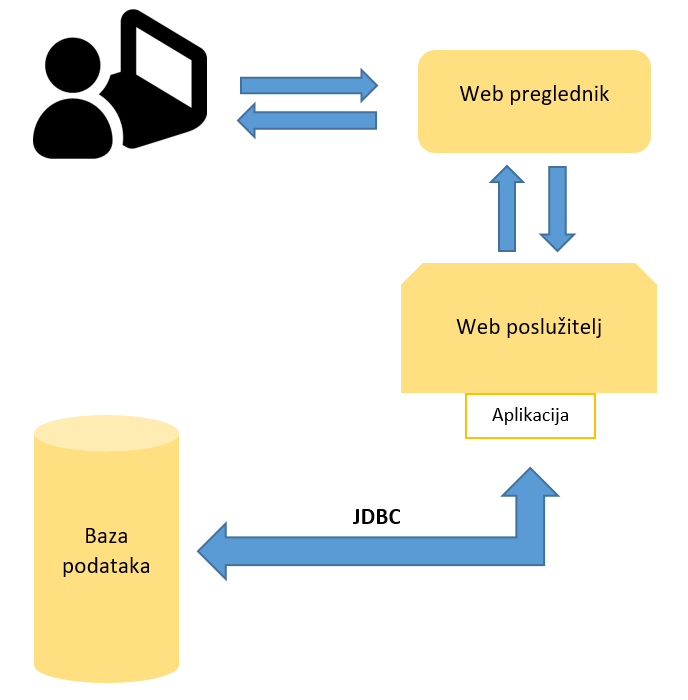
\includegraphics[scale=0.8]{arhitektura/arhitektura_sustava.png} %veličina slike u odnosu na originalnu datoteku i pozicija slike
					\centering
					\caption{Arhitektura sustava}
					\label{fig:arhitektura}
		\end{figure}

	\vspace{5mm} %5mm vertical space

		Web aplikacija će se temeljiti na modelu klijent-poslužitelj, što je danas i najčešće korišteni model. Korisnik šalje zahtjeve na koje odgovara poslužitelj, dok i jedna i druga strana mogu imati korisničku i poslužiteljsku aplikaciju.

	\vspace{10mm} %10mm vertical space

		\textbf{\underline{Web preglednik:} }\\

			Klijentski program, zvan preglednik, služi kao korisničko sučelje za pregledavanje sadržaja na Webu. On je taj koji šalje zahtjev Web poslužitelju i prikazuje primljene podatke u obliku Web stranica korisniku. Dakle, preglednik će primljene podatke u obliku koda interpretirati u nešto korisniku razumljivo, odnosno prikazat će korisničko sučelje naše aplikacije. Konačan prikaz aplikacije može uključivati više dohvata resursa i često može sadržavati dodatke te pomoćne aplikacije za prikaz formata koje izvorno ne podržava.

		\vspace{5mm} %5mm vertical space
		\textbf{\underline{Web poslužitelj:} }\\

		Poslužiteljski program poslužuje resurse smještene na poslužiteljskom računalu ili na drugim izvorima i odgovara na zahtjeve korisnika. Komunikacija se odvija preko HTTP/HTTPS (\textit{HyperText Transfer Protocol/Secure}) standardnog internetskog aplikacijskog protokola koji ima mogućnost prijenosa raznih vrsta podataka i proširiv je prema novim formatima podataka. Poslužitelj je zaslužan za pokretanje Web aplikacije.

		\vspace{5mm} %5mm vertical space
		
		\textbf{\underline{Web aplikacija:} }\\

		Za realizaciju frontend-a, odnosno korisničkog sučelja upotrijebit ćemo React kao bazu unutar kojega ćemo koristiti jezike HTML, TypeScript i CSS. TypeScript nam omogućava izradu dinamičkih web stranica u kombinaciji s HTML-om i CSS-om i njime možemo mijenjati sadržaj na stranici ovisno o načinu interakcije korisnika sa stranicom. Uz ove navedene tehnologije moguće je napraviti moderno korisničko sučelje jedne Web i mobilne aplikacije. Nakon što Web preglednik korisniku prikaže aplikaciju ''Planinarski dnevnik'', korisnik može izvršiti određenu naredbu odabirom neke od funkcionalnosti aplikacije. Hoće li pristupiti bazi podataka ovisi o samoj akciji. Za komunikaciju s bazom podataka koristi se JDBC koji predstavlja sučelje aplikacijskog programiranja za jezik Java i definira kako klijent može pristupiti bazi podataka. Pruža metode za upit i ažuriranje u bazi podataka te je orijentiran prema relacijskim bazama podataka. Što se tiče backend-a koristimo Spring Boot i MVC arhitekturu. 


		\vspace{5mm} %5mm vertical space

		\textbf{Spring Boot} pruža fleksibilan način konfiguriranja Java Beans, XML konfiguracija i transakcija baze podataka te bitno olakšava upravljanje ovisnostima. Svaka pokrenuta usluga ima svoj postupak, a time se postiže jednostavan model za podršku aplikacijama.  


		\vspace{5mm} %5mm vertical space

		\textbf{Model – View – Controller} je obrazac koji razdvaja aplikaciju u tri glavne logičke komponente: Model, View i Controller. Svaka od nabrojenih komponenti ima zadatak rukovati s određenim razvojnim aspektima aplikacije. Također, one su nezavisne jedna od druge i kao rezultat toga je jednostavno dodavanje i preoblikovanje svojstava.


		\vspace{5mm} %5mm vertical space

		\begin{itemize}
		\item \textbf{Model}	
		
		Poznat je kao najniža razina što znači da je odgovoran za održavanje podataka s kojima korisnik radi. Glavni zadatak je dohvat, manipulacija podatcima i uglavnom on surađuje s bazom podataka. Reagira na zahtjeve Controller-a jer on nikada sam ne razgovara s bazom podataka i nakon komunikacije prosljeđuje potrebne podatke Controllor-u. Jedna od bitnijih stvari za napomenuti je da Model nikada izravno ne komunicira s View.

		\item \textbf{View}
		
		Služi za prikazivanje podataka na način da zapravo generira korisničko sučelje za korisnika. Ti podaci su rezultat rada Model-a, ali se oni ne preuzimaju izravno već putem Controller-a tako da View surađuje samo s Controller-om. 

		\item \textbf{Controller}

		Djeluje u službi posrednika između komponenti Model i View. Ne mora brinuti o rukovanju logikom podataka, već samo govori Model-u što treba učiniti. Nakon primanja podataka od Model-a, on ih obrađuje i konačno rezultat prosljeđuje do View-a gdje objašnjava kako ih prikazati korisniku. Ako je došlo do promjena, Controller je zadužen za ažuriranje View-a.


		\end{itemize}


		\begin{figure}[H]
					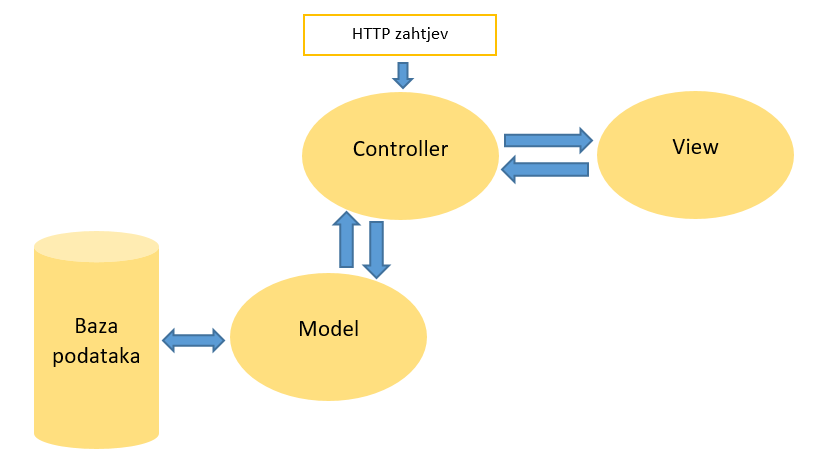
\includegraphics[scale=0.8]{arhitektura/mvc.png} %veličina slike u odnosu na originalnu datoteku i pozicija slike
					\centering
					\caption{Model - View - Controller}
					\label{fig:arhitektura}
		\end{figure}

		\section{Baza podataka}
			
		Za naš projekt odabrali smo \textbf{relacijsku bazu podataka} zbog njezine pogodnosti da prikaže mali dio stvarnog svijeta bez redundancije unutar same baze. Dohvaćanje podataka je relativno brzo i lagano se može paralelizirati. Specifičnu implementaciju relacijske baze podataka koju smo odabrali je \textbf{PostgreSQL}. To je baza podataka otvorenog koda s preko 30 godina aktivnog razvoja zbog kojeg je zaslužila svoju čvrstu reputaciju za pouzdanost, bogatstvo opcijama i visokim performansama. Zbog načina na koji je SQL standard napisan, vrlo je slična ostalim SQL bazama podataka.\\ 
		
		Tijekom razvoja koristimo \textbf{H2 bazu}. To je privremena baza podataka koja služi za testiranje koda. Svi zapisi u njoj se nalaze u privremenoj memoriji i nisu perzistentni. Zbog toga je odlična za testiranje. Ona je otvorenog koda, napisana u Javi i ima čvrste sigurnosne postavke. Na nju se možemo povezati s više konekcija i baza podataka je enkriptirana SHA-256 enkripcijom. Ima vrlo malu potrošnju memorije i zauzima relativno malo prostora na disku (oko 2MB). \\ 
		
		Također koristimo \textbf{JPA (Java Persistence API)} koje samo sadrži sučelja za stvaranje Persistence layouta. Dopušta nam da mapiramo entitete tablica i veze između tablica na objekte u Javi. Ovo sučelje definira svoj vlastiti jezik za upite (JPQA). JPQA prevoditelj interpretira kod i piše SQL upite. JPA ne možemo samostalno koristiti, već nam treba konkretna implementacija toga sučelja. Implementacija koju ćemo mi koristiti se zove Hibernate. \\ 
		
		Na bazu podataka se iz Jave spajamo preko \textbf{JdbcTemplatea}. To je snažni mehanizam za spajanje i izvođenje SQL upita. On nam smanjuje količinu koda koju moramo napisati kako bismo izvršavali upite, kao što je spajanje na bazu, kreiranje izraza i zatvaranje konekcija. \\
		\newpage
	Naš model baze podataka sastoji se od sljedećih \textbf{glavnih} i \underline{veznih} tablica:
		\begin{itemize}[noitemsep]
		\item \textbf{user}
		\item \textbf{residence$\_$place}
		\item \textbf{role}
		\item \textbf{mountain$\_$lodge}
		\item \textbf{mountain$\_$path}
		\item \textbf{event}
		\item \textbf{hill}
		\item \textbf{utility}
		\item \textbf{badge}
		\item \textbf{contact$\_$message}
		\item \underline{friendships}
		\item \underline{frienship$\_$req}
		\item \underline{user$\_$role}
		\item \underline{user$\_$place}
		\item \underline{user$\_$badge}
		\item \underline{mountain$\_$lodge$\_$utility}
		\item \underline{mountain$\_$lodge$\_$report}
		\item \underline{event$\_$path}
		\item \underline{event$\_$attendance}
		\item \underline{mountain$\_$path$\_$report}
		\item \underline{mountain$\_$path$\_$grade}
		\item \underline{path$\_$user$\_$wishlist}
		\item \underline{mountain$\_$path$\_$completed}
		\item \underline{badge\_notification}

\end{itemize}
		 \newpage
			\subsection{Opis tablica}
			Primarni ključevi su označeni \textbf{podebljano}, dok su strani ključevi \underline{podvučeni}. \\
			Prikazane su i sve vezne tablice, tako da se nad glavnim tablicama Many-To-Many veze neće navoditi.
			
%Tablice
			\textbf{user} -  ovaj entitet sadrži sve važne informacije o korisniku aplikacije.
			Sadrži atribute: "id", "full$\_$name", "email", "password", "image", "id$\_$place", "date$\_$of$\_$birth" i "description" koji redom predstavljaju jedinstveni identifikacijski broj korisnika, ime i prezime, e-mail korisnika, lozinku korisnika, sliku vidljivu na profilu korisnika, identifikacijski broj mjesta stanovanja korisnika te datum rođenja korisnika.
			Neki podaci o korisniku, kao što su mjesto stanovanja i datum rođenja su opcionalni, i ako ih korisnik ne ispuni njihova vrijednost je \textit{NULL}. Atribut "place\_id" je strani ključ koji referencira entitet \textbf{residence\_place} te se radi o Many-To-One vezi. 
			
			\begin{longtabu} to \textwidth {|X[6, l]|X[6, l]|X[20, l]|}
				\hline \multicolumn{3}{|c|}{\textbf{user - (Korisnik)}}	 \\[3pt] \hline
				\endfirsthead
				
				\hline \multicolumn{3}{|c|}{\textbf{user - (Korisnik)}}	 \\[3pt] \hline
				\endhead
				
				\hline 
				\endlastfoot
				
				\textbf{id} & BIGINT	&  	jedinstveni identifikacijski broj korisnika	\\ \hline
				full$\_$name	& VARCHAR &  ime i prezime korisnika 	\\ \hline 
				email & VARCHAR &  e-mail pomoću kojeg se korisnik prijavljuje u sustav \\ \hline 
				password & VARCHAR	&  	lozinka pomoću koje se korisnik prijavljuje u sustav	\\ \hline 
				image & BYTEA	&  	slika vidljiva na profilu korisnika	\\ \hline 
				\underline{place\_id} & BIGINT & strani ključ mjesta stanovanja korisnika iz tablice \textbf{residence\_place}, unos je opcionalan\\ \hline
				date\_of\_birth & DATE & datum rođenja korisnika, unos je opcionalan \\ \hline
				
				
			\end{longtabu}
			\vspace{10mm}
			
			\textbf{residence\_place}  Ovo je entitet koji modelira mjesto stanovanja korisnika. Sadrži atribute: "id" i "name" koji predstavljaju jedinstveni identifikator mjesta te naziv mjesta.
			
			
			\begin{longtabu} to \textwidth {|X[6, l]|X[6, l]|X[20, l]|}
				
				\hline \multicolumn{3}{|c|}{\textbf{residence\_place - (Mjesto stanovanja)}}	 \\[3pt] \hline
				\endfirsthead
				
				\hline \multicolumn{3}{|c|}{\textbf{residence\_place - (Mjesto stanovanja)}}	 \\[3pt] \hline
				\endhead
				
				\hline 
				\endlastfoot
				
				\textbf{id} & BIGINT	&  	jedinstveni indetifikacijski broj mjesta stanovanja	\\ \hline
				name	& VARCHAR &  naziv mjesta 	\\ \hline 
				%\cellcolor{LightBlue} primjer	& VARCHAR &   	\\ \hline 
				
				
			\end{longtabu}
				
				\vspace{10mm}
			\newpage
			\textbf{role} Ovaj entitet modelira ulogu korisnika unutar aplikacije, tzv. "aplikativne role". Određuje razinu ovlasti koje korisnik ima. Sadrži atribute: "id" i "name" koji predstavljaju jedinstveni identifikator uloge te naziv uloge. Dopuštene uloge u našoj aplikaciji su: Planinar, Dežurni planinar i Administrator.
			
			\begin{longtabu} to \textwidth {|X[6, l]|X[6, l]|X[20, l]|}
				
				\hline \multicolumn{3}{|c|}{\textbf{role - (Uloga)}}	 \\[3pt] \hline
				\endfirsthead
				
				\hline \multicolumn{3}{|c|}{\textbf{role - ime tablice}}	 \\[3pt] \hline
				\endhead
				
				\hline 
				\endlastfoot
				
				\textbf{id} & BIGINT	&  jedinstveni ID uloge	\\ \hline
				name	& VARCHAR &  ime uloge 	\\ \hline 
				
			\end{longtabu}
		
		\vspace{10mm}		
		
		\textbf{mountain\_lodge} Ovaj entitet modelira jedan planinarski dom. Sadrži atribute: "id", "name", "image", "elevation" i "hill\_id" koji predstavljaju jedinstveni identifikator planinarskog doma, naziv planinarskog doma, sliku planinarskog doma, nadmorsku visinu te jedinstveni identifikator zemljopisnog područja (visočja) na kojemu se planinarski dom nalazi. Unos slike za neki planinarski dom je opcionalan, a ako se atribut ne popuni njegova vrijednost je \textit{NULL}. Atribut "hill\_id" predstavlja strani ključ koji referencira entitet \textbf{hill} te se radi o Many-To-One vezi. 
		
		\begin{longtabu} to \textwidth {|X[6, l]|X[6, l]|X[20, l]|}
			
			\hline \multicolumn{3}{|c|}{\textbf{mountain\_lodge - (Planinarski dom)}}	 \\[3pt] \hline
			\endfirsthead
			
			\hline \multicolumn{3}{|c|}{\textbf{mountain\_lodge - ime tablice}}	 \\[3pt] \hline
			\endhead
			
			\hline 
			\endlastfoot
			
			\textbf{id} & BIGINT	&  	jedinstveni identifikacijski broj planinarskog doma 	\\ \hline
			name	& VARCHAR &   naziv planinarskog doma	\\ \hline 
			image & BYTEA &  slika planinarskog doma koja se prikazuje unutar aplikacije, unos je opcionalan \\ \hline 
			elevation & INTEGER & nadmorska visina na kojoj se planinarski dom nalazi izražena u kilometrima \\ \hline 
			\underline{hill\_id} & BIGINT	&  strani ključ na tablicu \textbf{hill}, a predstavlja identifikator visočja na kojemu se nalazi planinarski dom	\\ \hline 
			
			
		\end{longtabu}
	\vspace{10mm}		
	
	
	\textbf{utility} Ovaj entitet modelira značajke infrastrukture pojedinog doma. Sadrži atribute "id" i "name" koji predstavljaju jedinstveni identifikacijski broj značajke te naziv značajke. Primjeri takvih značajki su pitka voda, hrana, smještaj, internet.
	
	\newpage
	\begin{longtabu} to \textwidth {|X[6, l]|X[6, l]|X[20, l]|}
		
		\hline \multicolumn{3}{|c|}{\textbf{utility - (Pogodnost, značajka)}}	 \\[3pt] \hline
		\endfirsthead
		
		\hline \multicolumn{3}{|c|}{\textbf{utility - ime tablice}}	 \\[3pt] \hline
		\endhead
		
		\hline 
		\endlastfoot
		
		\textbf{id} & BIGINT	&  jedinstveni identifikator značajke\\ \hline
		name	& VARCHAR &  naziv značajke/pogodnosti \\ \hline 
		
	\end{longtabu}
				\vspace{10mm}		
				
				\textbf{hill} Ovaj entitet modelira pojedino zemljopisno područje, odnosno visočje na kojemu se nalazi pojedini planinarski dom ili planinarska staza. Sadrži atribute: "id" i "name" koji predstavljaju jedinstveni identifikacijski broj visočja te naziv visočja.
				
				\begin{longtabu} to \textwidth {|X[6, l]|X[6, l]|X[20, l]|}
					
					\hline \multicolumn{3}{|c|}{\textbf{hill - (Visočje)}}	 \\[3pt] \hline
					\endfirsthead
					
					\hline \multicolumn{3}{|c|}{\textbf{hill - ime tablice}}	 \\[3pt] \hline
					\endhead
					
					\hline 
					\endlastfoot
					
					\textbf{id} & BIGINT	&  jedinstveni ID visočja 	\\ \hline
					name & VARCHAR	&  ime visočja 	\\ \hline
					
					
				\end{longtabu}
				\vspace{10mm}
			
			\textbf{mountain\_path} Ovaj entitet sadrži informacije o pojedinoj planinarskoj stazi. Sadrži atribute: "id", "name", "start\_point", "end\_point", "avg\_walk\_time", "length", "sea\_level\_diff", "date\_created", "is\_private", "author\_id" i "hill\_id" koji redom predstavljaju jedinstveni identifikacijski broj planinarske staze, naziv staze, polazišnu točku, završnu toku, prosječno vrijeme potrebno da se prepješači staza, duljinu staze, razliku u nadmorskoj visini između početne i završne točke, datum kreiranja pojedine staze od strane korisnika unutar naše aplikacije, vrijednost koja govori je li staza privatna ili javna, korisnika koji je stvorio stazu te identifikator visočja na kojemu se staza nalazi. Atribut "author\_id" te atribut "hill\_id" su strani ključevi obzirom na tablicu \textbf{user} odnosno \textbf{hill} te se radi o Many-To-One vezama.
			
			\begin{longtabu} to \textwidth {|X[6, l]|X[6, l]|X[20, l]|}
				
				\hline \multicolumn{3}{|c|}{\textbf{mountain\_path - (Planinarska staza)}}	 \\[3pt] \hline
				\endfirsthead
				
				\hline \multicolumn{3}{|c|}{\textbf{mountain\_path - (Planinarska staza)}}	 \\[3pt] \hline
				\endhead
				
				\hline 
				\endlastfoot
				
				\textbf{id} & BIGINT	& jedinstveni identifikacijski broj planinarske staze	\\ \hline
				name	& VARCHAR &  naziv staze	\\ \hline 
				start\_point & VARCHAR & naziv početne točke staze  \\ \hline 
				end\_point & VARCHAR &  naziv završne točke staze \\ \hline 
				avg\_walk\_time & TIME &  prosječno vrijeme potrebno za prepješačiti stazu\\ \hline 
				length & INTEGER & duljina staze u metrima\\ \hline 
				sea\_level\_diff & INTEGER & razlika u nadmorskoj visini između početne i završne točke staze\\ \hline 
				date\_created & DATE &  datum stvaranja staze unutar aplikacije\\ \hline 
				is\_private & BOOLEAN	&  atribut koji govori je li korisnik stazu stvara privatno ili javno  \\ \hline 
				\underline{author\_id} & BIGINT	&  	identifikacijski broj korisnika koji je stvorio stazu unutar aplikacije\\ \hline 
				\underline{hill\_id} & BIGINT	&  identifikacijski broj visočja na kojemu se staza nalazi\\ \hline 
				
				
			\end{longtabu}
			\vspace{10mm}
			
			\textbf{event} Ovaj entitet modelira jedan događaj koji stvara korisnik unutar naše aplikacije. Jedan događaj počinje u određeno vrijeme "start\_date", te završava u određeno vrijeme: "end\_date". Svaki događaj, odnosno planinarski izlet sastoji se od jedne ili više planinarskih staza koje se obilaze tijekom tog planinarskog izleta. Osim toga, planinarski izlet ima svoj opis: "description", gdje korisnik može reći više pojedinosti o samom planinarskom izletu. Osim toga, ovaj entitet sadrži atribute: "id", "name", "date\_created" i "author\_id" koji predstavljaju jedinstveni identifikacijski broj događaja, naziv događaja, vrijeme kada je korisnik stvorio događaj unutar aplikacije te jedinstveni identifikacijski broj korisnika koji je stvorio događaj. Atribut "author\_id" je strani ključ koji se odnosi na tablicu \textbf{user} te se radi o Many-To-One vezi.
			
			\begin{longtabu} to \textwidth {|X[6, l]|X[6, l]|X[20, l]|}
				
				\hline \multicolumn{3}{|c|}{\textbf{event - (Planinarski događaj)}}	 \\[3pt] \hline
				\endfirsthead
				
				\hline \multicolumn{3}{|c|}{\textbf{event - (Planinarski događaj)}}	 \\[3pt] \hline
				\endhead
				
				\hline 
				\endlastfoot
				
				\textbf{id} & BIGINT	&  	jedinstveni identifikacijski broj planinarskog izleta 	\\ \hline
				name	& VARCHAR & naziv događaja 	\\ \hline 
				description & VARCHAR &  pojedinosti vezane uz događaj \\ \hline 
				start\_date & TIMESTAMP	&  vrijeme i datum početka planinarskog izleta	\\ \hline 
				end\_date & TIMESTAMP	&  	vrijeme i datum završetka planinarskog izleta	\\ \hline 
				date\_created & TIMESTAMP	&  vrijeme i datum stvaranja izleta unutar aplikacije\\ \hline 
				\underline{author\_id} & BIGINT	& jedinstveni identifikacijski broj korisnika koji je stvorio događaj unutar aplikacije		\\ \hline 
				
				
			\end{longtabu}
			\vspace{10mm}
			
			\textbf{badge} Ovaj entitet modelira jedan bedž, odnosno priznanje koje korisnik može zaslužiti kao planinar. Korisnik priznanja zaslužuje za svoju aktivnost koja se gleda na osnovu arhive planinarskih domova i staza, te se uzimaju u obzir značajke kao što su: broj posjećenih planinarskih domova, broj odrađenih planinarskih staza i sl. Entitet sadrži atribute "id" i "name" koji predstavljaju jedinstveni identifikacijski broj priznanja te naziv priznanja.
			
			\begin{longtabu} to \textwidth {|X[6, l]|X[6, l]|X[20, l]|}
				
				\hline \multicolumn{3}{|c|}{\textbf{badge - (Priznanje)}}	 \\[3pt] \hline
				\endfirsthead
				
				\hline \multicolumn{3}{|c|}{\textbf{badge - (Priznanje)}}	 \\[3pt] \hline
				\endhead
				
				\hline 
				\endlastfoot
				
				\textbf{id}	& BIGINT &   jedinstveni identifikacijski broj priznanja	\\ \hline 
				name & VARCHAR &  naziv priznanja \\ \hline 
				
				
			\end{longtabu}
		
				\vspace{10mm}
				
				\textbf{contact\_message} Ovaj entitet modelira poruke koje korisnik može slati administratoru u slučaju npr. otvaranja novog planinarskog doma. Sadrži atribute: "id", "description", "date\_send" koji redom predstavljaju jedinstveni identifikacijski broj poruke, opis odnosno sadržaj poruke te datum i vrijeme slanja poruke.
				
				\begin{longtabu} to \textwidth {|X[6, l]|X[6, l]|X[20, l]|}
					
					\hline \multicolumn{3}{|c|}{\textbf{contact\_message - (Poruke administratoru)}}	 \\[3pt] \hline
					\endfirsthead
					
					\hline \multicolumn{3}{|c|}{\textbf{badge - (Priznanje)}}	 \\[3pt] \hline
					\endhead
					
					\hline 
					\endlastfoot
					
					\textbf{id}	& BIGINT &   jedinstveni identifikacijski broj poruke	\\ \hline 
					description & VARCHAR &  sadržaj poruke \\ \hline 
					created\_on & DATE &  datum i vrijeme slanja poruke \\ \hline 
					\underline{user\_id} & BIGINT	& jedinstveni identifikacijski broj korisnika koji je stvorio poruku unutar aplikacije		\\ \hline 
					
				\end{longtabu}
				\vspace{10mm}
				
	
			\textbf{friendships} Ovo je vezna tablica koja sadrži Many-To-Many vezu između dva korisnika, a služi nam za modeliranje prijateljstava, odnosno pripadanja istoj planinarskoj zajednici. Sadrži atribute "user\_id1" i "user\_id2" koji predstavljaju strane ključeve na tablicu \textbf{user} i govore nam tko su korisnici koji pripadaju istoj zajednici, te atribut "friendship\_created" koji nam govori o datumu i vremenu stvaranja prijateljstva.
			
			\begin{longtabu} to \textwidth {|X[6, l]|X[6, l]|X[20, l]|}
				
				\hline \multicolumn{3}{|c|}{\textbf{friendships - (Prijatelji)}}	 \\[3pt] \hline
				\endfirsthead
				
				\hline \multicolumn{3}{|c|}{\textbf{friendships - (Prijatelji)}}	 \\[3pt] \hline
				\endhead
				
				\hline 
				\endlastfoot
				
				\underline{user\_id1} & BIGINT	&  strani ključ koji se odnosi na jednog korisnika člana veze "prijatelji"	\\ \hline
				\underline{user\_id2}	& BIGINT &   strani ključ koji se odnosi na drugog korisnika člana veze "prijatelji"\\ \hline 
				friendship$\_$ \text{created}	& TIMESTAMP &   vrijeme i datum kada su dva određena korisnika postala prijatelji	\\ \hline 
				%\cellcolor{LightBlue} primjer	& VARCHAR &   	\\ \hline 
				
				
			\end{longtabu}
			\vspace{10mm}

			\textbf{friendship\_req} Ovaj entitet sadrži informaciju o poslanom zahtjevu za prijateljstvo između 2 korisnika. Sadrži atribute: "friendship\_send" te "friendship\_recieve" koji su oba strani ključevi iz tablice \textbf{user}, a predstavljaju identifikacijski broj pošiljatelja te primatelja zahtjeva za prijateljstvo. Radi se o refleksivnoj Many-to-Many vezi.
			
			\begin{longtabu} to \textwidth {|X[6, l]|X[6, l]|X[20, l]|}
				
					\hline \multicolumn{3}{|c|}{\textbf{friendship\_req - (Zahtjevi za prijateljstvom)}}	 \\[3pt] \hline
				\endfirsthead
				
				\hline \multicolumn{3}{|c|}{\textbf{friendship\_req - (Zahtjevi za prijateljstvom)}}	 \\[3pt] \hline
				\endhead
				
				\hline 
				\endlastfoot
				
				\underline{friendship\_} \underline{send} & BIGINT	&  strani ključ korisnika koji šalje zahtjev za prijateljstvom iz tablice \textbf{user} 	\\ \hline
				\underline{friendship\_} \underline{recieve}	& BIGINT &   strani ključ korisnika koji prima zahtjev za prijateljstvom	iz tablice \textbf{user}\\ \hline 
				%\cellcolor{LightBlue} primjer	& VARCHAR &   	\\ \hline 
				
				
			\end{longtabu}
		\vspace{10mm}
		
		\textbf{user\_role} Vezna tablica koja modelira Many-to-Many vezu između entiteta \textbf{user} i entiteta \textbf{role}. Jedan korisnik može imati više uloga, dok jednu ulogu može imati više različitih korisnika. Sadrži atribute "role\_id" te "user\_id" koji redom predstavljaju identifikacijski broj uloge te identifikacijski broj korisinika.
		
		\begin{longtabu} to \textwidth {|X[6, l]|X[6, l]|X[20, l]|}
			
			\hline \multicolumn{3}{|c|}{\textbf{user\_role}}	 \\[3pt] \hline
			\endfirsthead
			
			\hline \multicolumn{3}{|c|}{\textbf{user\_role}}	 \\[3pt] \hline
			\endhead
			
			\hline 
			\endlastfoot
			
			\underline{user\_id} & BIGINT	&  	strani ključ korisnika iz entiteta \textbf{user}	\\ \hline
			\underline{role\_id}	& BIGINT &  strani ključ uloge, odnosno aplikativne role iz entiteta \textbf{role}\\ \hline 
			
			
		\end{longtabu}
			\vspace{10mm}
			
			\textbf{user\_badge} Ovaj entitet sadrži informaciju o Many-To-Many odnosu između bedževa (priznanja) i korisnika. Sadrži atribute: "user\_id", "badge\_id" i "date\_recieved" koji redom predstavljaju identifikacijski broj korisnika, identifikacijski broj priznanja te vrijeme dobivanja priznanja.
			
			\begin{longtabu} to \textwidth {|X[6, l]|X[6, l]|X[20, l]|}
				
				\hline \multicolumn{3}{|c|}{\textbf{user\_badge}}	 \\[3pt] \hline
				\endfirsthead
				
				\hline \multicolumn{3}{|c|}{\textbf{user\_badge}}	 \\[3pt] \hline
				\endhead
				
				\hline 
				\endlastfoot
				
				\underline{user\_id} & BIGINT	&  strani ključ korisnika kojem je pripisan pojedini bedž iz tablice \textbf{user}\\ \hline
				\underline{badge\_id}	& BIGINT &  strani ključ bedža kojeg je dobio pojedini korisnik iz tablice \textbf{badge}	\\ \hline 
				date\_recieved & DATE & datum dobivanja pojedinog bedža za određenog korisnika  \\ \hline 
				
				
			\end{longtabu}
			\vspace{10mm}

			\textbf{event\_attendance} Modelira Many-To-Many vezu između korisnika i događaja (planinarskog izleta) na kojemu korisnik želi sudjelovati. Sadrži atribute "user\_id" te "event\_id" koji predstavljaju jedinstveni identifikator korisnika koji sudjeluje na događaju te jedinstveni identifikator događaja.
			
			\begin{longtabu} to \textwidth {|X[6, l]|X[6, l]|X[20, l]|}
				
				\hline \multicolumn{3}{|c|}{\textbf{event\_attendance}}	 \\[3pt] \hline
				\endfirsthead
				
				\hline \multicolumn{3}{|c|}{\textbf{event\_attendance}}	 \\[3pt] \hline
				\endhead
				
				\hline 
				\endlastfoot
				
				\underline{user\_id} & BIGINT	&  	strani ključ korisnika koji će prisustvovati događaju iz tablice \textbf{user}	\\ \hline
				\underline{event\_id}	& BIGINT &  strani ključ događaja kojemu određena osoba pristupa iz tablice \textbf{event}\\ \hline 
				
				
			\end{longtabu}
			\vspace{10mm}		
			
			\textbf{event\_path} Ovaj entitet sadrži informaciju o Many-To-Many vezi između planinarske staze i nekog planinarskog događaja. Sadrži atribute: "path\_id" te "event\_id" koji predstavljaju identifikacijski broj planinarske staze i identifikacijski broj nekog planinarskog događaja. Osim toga, sadrži atribut "event\_day" koji nam govori o rednom broju dana tijekom kojeg se na određenom planinarskom događaju odrađuje određena planinarska staza.
			
			\begin{longtabu} to \textwidth {|X[6, l]|X[6, l]|X[20, l]|}
				
				\hline \multicolumn{3}{|c|}{\textbf{event\_path}}	 \\[3pt] \hline
				\endfirsthead
				
				\hline \multicolumn{3}{|c|}{\textbf{event\_path}}	 \\[3pt] \hline
				\endhead
				
				\hline 
				\endlastfoot
				
				\underline{path\_id} & BIGINT	&  	strani ključ staze koja je dio nekog događaja iz tablice \textbf{mountain\_path}	\\ \hline
				\underline{event\_id}	& BIGINT &  strani ključ događaja u kojem se pojedina staza odrađuje, iz tablice \textbf{event}	\\ \hline 
				event\_day	& INTEGER &  redni broj dana koliko se unutar jednog događaja obilazi određena staza	\\ \hline 
				
			\end{longtabu}
			\vspace{10mm}
		
			\textbf{badge\_notification} Ovaj entitet sadrži informaciju o Many-To-Many odnosu između bedževa i korisnika, ali samo u smislu obavijesti korisniku. Kada korisnik potvrdi da je primio obavijest, pojedini unos se briše iz ovog entiteta. Sadrži atribute: "user\_id" te "badge\_id" koji predstavljaju identifikator korisnika koji je dobio priznanje čiji je identifikator "badge\_id".
			
			\begin{longtabu} to \textwidth {|X[6, l]|X[6, l]|X[20, l]|}
				
				\hline \multicolumn{3}{|c|}{\textbf{badge\_notification}}	 \\[3pt] \hline
				\endfirsthead
				
				\hline \multicolumn{3}{|c|}{\textbf{badge\_notification}}	 \\[3pt] \hline
				\endhead
				
				\hline 
				\endlastfoot
				
				\underline{user\_id} & BIGINT	&  strani ključ korisnika kojem je pripisan pojedini bedž iz tablice \textbf{user}\\ \hline
				\underline{badge\_id}	& BIGINT) &  strani ključ bedža kojeg je dobio pojedini korisnik iz tablice \textbf{badge}\\ \hline  
				
				
			\end{longtabu}
			\vspace{10mm}		
		
			\textbf{mountain\_lodge\_utility} Vezna tablica koja modelira Many-to-Many vezu između planinarskih domova i infrastrukturnih značajki koje ti domovi posjeduju. Sadrži atribute "lodge\_id" te "utility\_id" koji predstavljaju identifikator planinarskog doma te identifikator odgovarajuće značajke.
			
			\begin{longtabu} to \textwidth {|X[6, l]|X[6, l]|X[20, l]|}
				
				\hline \multicolumn{3}{|c|}{\textbf{mountain\_lodge\_utility}}	 \\[3pt] \hline
				\endfirsthead
				
				\hline \multicolumn{3}{|c|}{\textbf{mountain\_lodge\_utility}}	 \\[3pt] \hline
				\endhead
				
				\hline 
				\endlastfoot
				
				\underline{lodge\_id} & BIGINT	&  strani ključ kojem je pripisan pojedini planinarski dom iz tablice  \textbf{mountain\_lodge}\\ \hline
				\underline{utility\_id}	& BIGINT &  strani ključ kojem je pripisana pojedina značajka iz tablice \textbf{utility} \\ \hline 
				
				
			\end{longtabu}
			\vspace{10mm}
			
			\textbf{mountain\_path\_grade} Vezna tablica koja nam govori o ocjenama koje pojedini korisnik dodijeljuje pojedinoj planinarskoj stazi. Radi se o Many-To-Many veznoj tablici. Sadrži atribute "user\_id", "path\_id" te "grade", koji redom predstavljaju identifikacijski broj korisnika, identifikacijski broj planinarske staze te ocjenu koju je taj korisnik dodijelio toj stazi.
			
			\begin{longtabu} to \textwidth {|X[6, l]|X[6, l]|X[20, l]|}
				
				\hline \multicolumn{3}{|c|}{\textbf{mountain\_path\_grade}}	 \\[3pt] \hline
				\endfirsthead
				
				\hline \multicolumn{3}{|c|}{\textbf{mountain\_path\_grade}}	 \\[3pt] \hline
				\endhead
				
				\hline 
				\endlastfoot
				
				\underline{user\_id} & BIGINT	& strani ključ korisnika koji daje ocjenu iz tablice \textbf{user}  	\\ \hline
				\underline{path\_id}	& BIGINT &   strani ključ planinarske staze koja se ocjenjuje iz tablice \textbf{mountain\_path}	\\ \hline 
				grade & INTEGER & ocjenu koju je korisnik dodijelio za konkretnu stazu  \\ \hline 
				
				
			\end{longtabu}
			\vspace{10mm}		
		
			\textbf{path\_user\_wishlist} Vezna tablica koja modelira željene planinarske staze za pojedinog korisnika. To su staze koje korisnik ima namjeru prepješačiti, ali još nije uspio. Sadrži atribute "user\_id" i "path\_id" koji predstavljaju identifikator korisnika te identifikator staze koju korisnik želi prepješačiti.
		
			\begin{longtabu} to \textwidth {|X[6, l]|X[6, l]|X[20, l]|}
				
				\hline \multicolumn{3}{|c|}{\textbf{path\_user\_wishlist}}	 \\[3pt] \hline
				\endfirsthead
				
				\hline \multicolumn{3}{|c|}{\textbf{path\_user\_wishlist}}	 \\[3pt] \hline
				\endhead
				
				\hline 
				\endlastfoot
				
				\underline{user\_id} & BIGINT	& strani ključ korisnika  koji želi prepješačiti neku stazu iz tablice \textbf{user}	\\ \hline
				\underline{path\_id} & BIGINT	& strani ključ staze koju korisnik želi prepješačiti iz tablice \textbf{mountain\_path}	\\ \hline
				
				
			\end{longtabu}
			\vspace{10mm}			
			
			\textbf{mountain\_path\_completed} Ovaj entitet sadrži informaciju o Many-To-Many odnosu između pojedinog korisnika i staza koje je već prepješačio, odnosno ovaj entitet modelira arhivu staza.
			
			\begin{longtabu} to \textwidth {|X[6, l]|X[6, l]|X[20, l]|}
				
				\hline \multicolumn{3}{|c|}{\textbf{mountain\_path\_completed}}	 \\[3pt] \hline
				\endfirsthead
				
				\hline \multicolumn{3}{|c|}{\textbf{mountain\_path\_completed}}	 \\[3pt] \hline
				\endhead
				
				\hline 
				\endlastfoot
				
				\underline{user\_id} & BIGINT	& strani ključ korisnika  koji je prepješačio pojedinu stazu iz tablice \textbf{user}	\\ \hline
				path\_id	& BIGINT &   strani ključ staze koju je konkretni korisnik prepješačio iz tablice \textbf{mountain\_path}	\\ \hline 
				date\_completed & DATE & datum kojeg je određeni korisnik prepješačio određenu stazu  \\ \hline 
				
				
			\end{longtabu}
			\vspace{10mm}
		
			\textbf{mountain\_path\_report} Vezna tablica koja modelira prijavu netočnih ili nepreciznih informacija vezanih uz pojedinu planinarsku stazu. Korisnik kojem je identifikacijski broj "user\_id" prijavljuje netočne informacije vezane uz planinarsku stazu identifikatora "path\_id", a osim toga bilježi se i vrijeme prijave pogreške kao atribut "date\_report", opis pogreške kao atribut "description" te status pogreške kao atribut "status" koji označava je li administrator pogrešku prihvatio, odbio ili je ona i dalje aktivna.
			\begin{longtabu} to \textwidth {|X[6, l]|X[6, l]|X[20, l]|}
				
				\hline \multicolumn{3}{|c|}{\textbf{mountain\_path\_report}}	 \\[3pt] \hline
				\endfirsthead
				
				\hline \multicolumn{3}{|c|}{\textbf{mountain\_path\_report}}	 \\[3pt] \hline
				\endhead
				
				\hline 
				\endlastfoot
				
				\underline{user\_id} & BIGINT	& strani ključ korisnika  koji prijavljuje netočnu ili nepreciznu informaciju vezanu uz neku planinarsku stazu, a odnosi se na tablicu \textbf{user}	\\ \hline
				\underline{path\_id}	& BIGINT &   strani ključ planinarske staze koju korisnik prijavljuje, a odnosi se na tablicu \textbf{mountain\_path}	\\ \hline 
				description & VARCHAR & opis netočne ili neprecizne informacije o nekoj stazi  \\ \hline 
				status & VARCHAR & status prijavljene pogreške  \\ \hline
				date\_report & TIMESTAMP & vrijeme i datum prijave pogreške vezane uz određenu planinarsku stazu  \\ \hline
				
		
				
				
			\end{longtabu}
					\vspace{10mm}
		
		\textbf{mountain\_lodge\_report} Vezna tablica koja modelira prijavu netočnih ili nepreciznih informacija vezanih uz pojedini planinarski dom. Korisnik kojem je identifikacijski broj "user\_id" prijavljuje netočne informacije vezane uz planinarski dom identifikatora "lodge\_id", a osim toga bilježi se i vrijeme prijave pogreške kao atribut "date\_report", opis pogreške kao atribut "description" te status pogreške kao atribut "status" koji označava je li administrator pogrešku prihvatio, odbio ili je ona i dalje aktivna.
		\begin{longtabu} to \textwidth {|X[6, l]|X[6, l]|X[20, l]|}
			
			\hline \multicolumn{3}{|c|}{\textbf{mountain\_lodge\_report}}	 \\[3pt] \hline
			\endfirsthead
			
			\hline \multicolumn{3}{|c|}{\textbf{mountain\_lodge\_report}}	 \\[3pt] \hline
			\endhead
			
			\hline 
			\endlastfoot
			
			\underline{user\_id} & BIGINT	& strani ključ korisnika  koji prijavljuje netočnu ili nepreciznu informaciju vezanu uz neki planinarski dom, a odnosi se na tablicu \textbf{user}	\\ \hline
			\underline{lodge\_id}	& BIGINT &   strani ključ planinarskog doma koji korisnik prijavljuje, a odnosi se na tablicu \textbf{mountain\_lodge}	\\ \hline 
			description & VARCHAR & opis netočne ili neprecizne informacije o nekom planinarskom domu  \\ \hline 
			status & VARCHAR & status prijavljene pogreške  \\ \hline
			date\_report & VARCHAR & vrijeme i datum prijave pogreške vezane uz određeni planinarski dom  \\ \hline
			
			
			
			
		\end{longtabu}
			\vspace{10mm}


			\subsection{Dijagram baze podataka}
				
				\begin{figure}[H]
					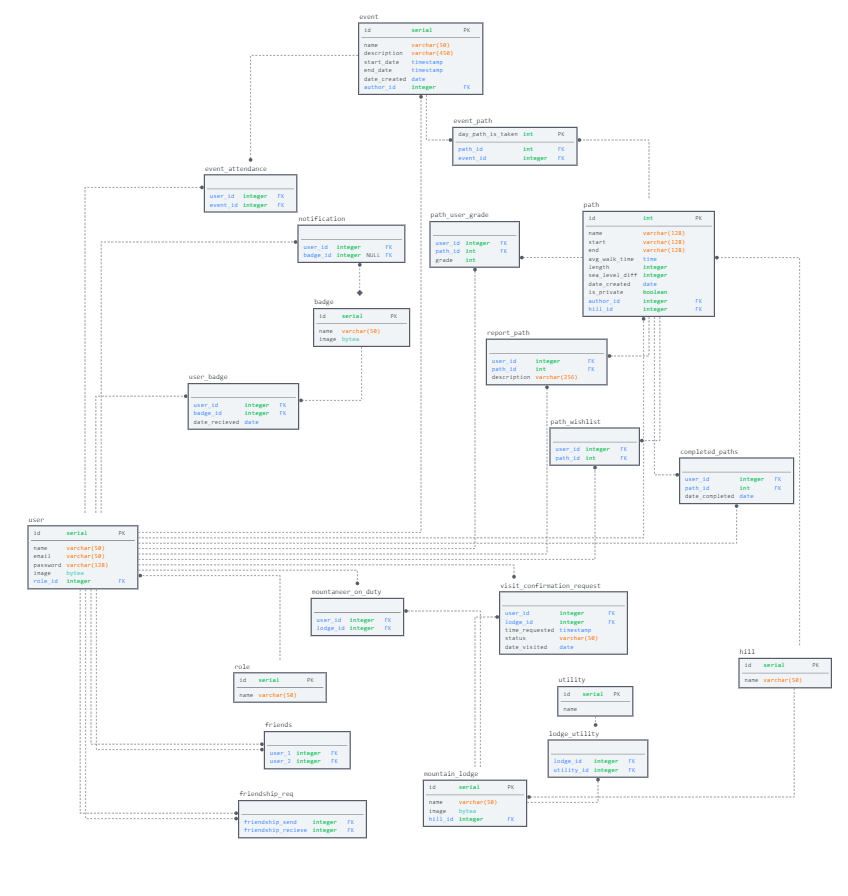
\includegraphics[scale=0.4, height=180mm]{slike/database.png} %veličina slike u odnosu na originalnu datoteku i pozicija slike
					\centering
					\caption{Dijagram baze podataka}
					\label{fig:dijagrambp}
				\end{figure}
			
			\eject
			
			
		\section{Dijagram razreda}
		
			\subsection{Konceptualni model dijagrama razreda}
			Prvi prikazani dijagram je konceptualni model dijagrama razreda. Na njemu su idejno prikazani razredi, njihove funkcionalnosti te odnosi između razreda. Svi razredi napravljeni su obzirom na obrasce uporabe i opise funkcionalnih zahtjeva.
		
			\begin{figure}[H]
				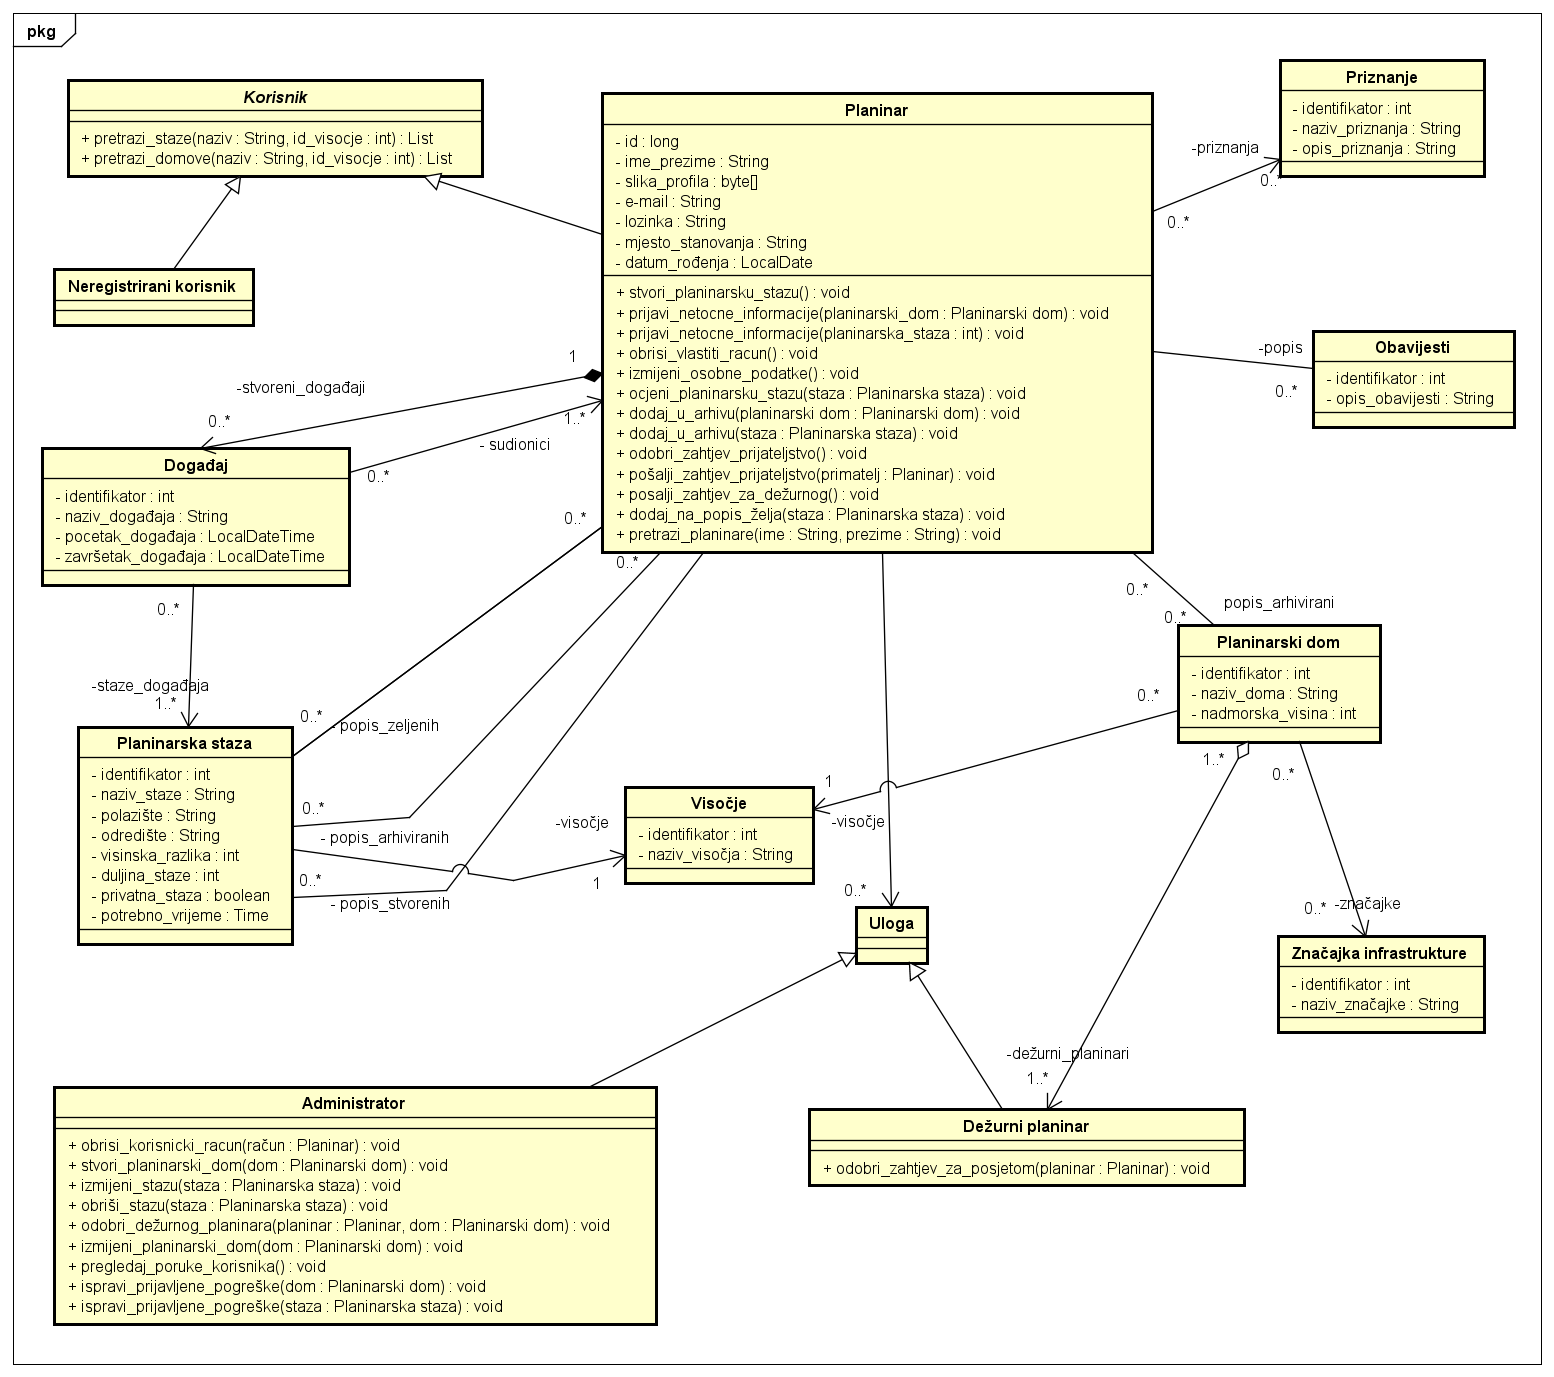
\includegraphics[scale=0.4, height=170mm, width=165mm]{dijagrami/domena-konceptualni.png} %veličina slike u odnosu na originalnu datoteku i pozicija slike
				\centering
				\caption{Dijagram razreda - konceptualni model}
				\label{fig:dijagrami_razreda3}
			\end{figure}
			
			\eject
			
			\subsection{Implementacijski dijagrami razreda - model sustava}
			\subsubsection{Sloj modela i objekti prijenosa podataka (DTO)}
			Na ovom dijagramu prikazan je sloj modela te su prikazani objekti prijenosa podataka, tzv. \textit{Data Transfer Objects}. Ovaj dijagram modela odnosi se na modele sustava koji su trenutno implementirani i koji omogućuju generičke funkcionalnosti potrebne za prvu predaju. U daljnjem radu i razvitku ovaj dijagram će se nadopunjavati sve do konačnog modela sustava. Možemo reći da je glavni razred na dijagramu razred \textit{User}, koji predstavlja registriranog korisnika aplikacije, odnosno planinara. On je povezan s razredom \textit{Role}, na način da svaki korisnik može imati više aplikativnih uloga, npr. ulogu \textit{Admin} ili \textit{Dežurni planinar}, međutim funkcionalnosti vezane uz te uloge još nisu implementirane. Vidimo i razred \textit{MountainLodge} koji modelira jedan planinarski dom. Planinarski dom može imati više značajki infrastrukture, što je na dijagramu prikazano vezom razreda \textit{MountainLodge} s razredom \textit{Utility}. Planinarski dom se isključivo nalazi na jednom visočju, koje je modelirano razredom \textit{Hill}. Osim tih razreda prikazani su DTO razredi: \textit{HillFindResponse}, \textit{UserCreateDto}, \textit{MountainLodgeSearchRequest}, \textit{MountainLodgeSearchResponse} te \textit{PageSearchResponse}. To su razredi koji služe za prijenos podataka i omogućavaju da nadglednik nikada ne radi sa stvarnim modelima. Osim njih, prikazano je sučelje \textit{DefaultMapper} kojeg implementiraju konkretni razredi za mapiranje, čija je dužnost mapirati razrede prijenosa podataka u modele i obrnuto. Za razrede modela prikazane su metode, dok za DTO objekte metode nisu prikazane zbog preglednosti.
			\begin{figure}[H]
				\includegraphics[scale=0.6, height=190mm, width=165mm]{dijagrami/model-DTO-sloj.png} %veličina slike u odnosu na originalnu datoteku i pozicija slike
				\centering
				\caption{Dijagram razreda - sloj modela i DTO}
				\label{fig:dijagrami_razreda2}
			\end{figure}
			\newpage
			\subsubsection{Daljnja idejna razrada sloja modela}
			Na sljedećem dijagramu idejno su prikazani prethodni modeli s novim metodama i razredi koji će se razvijati u narednim iteracijama razvoja projekta. 
			\begin{figure}[H]
				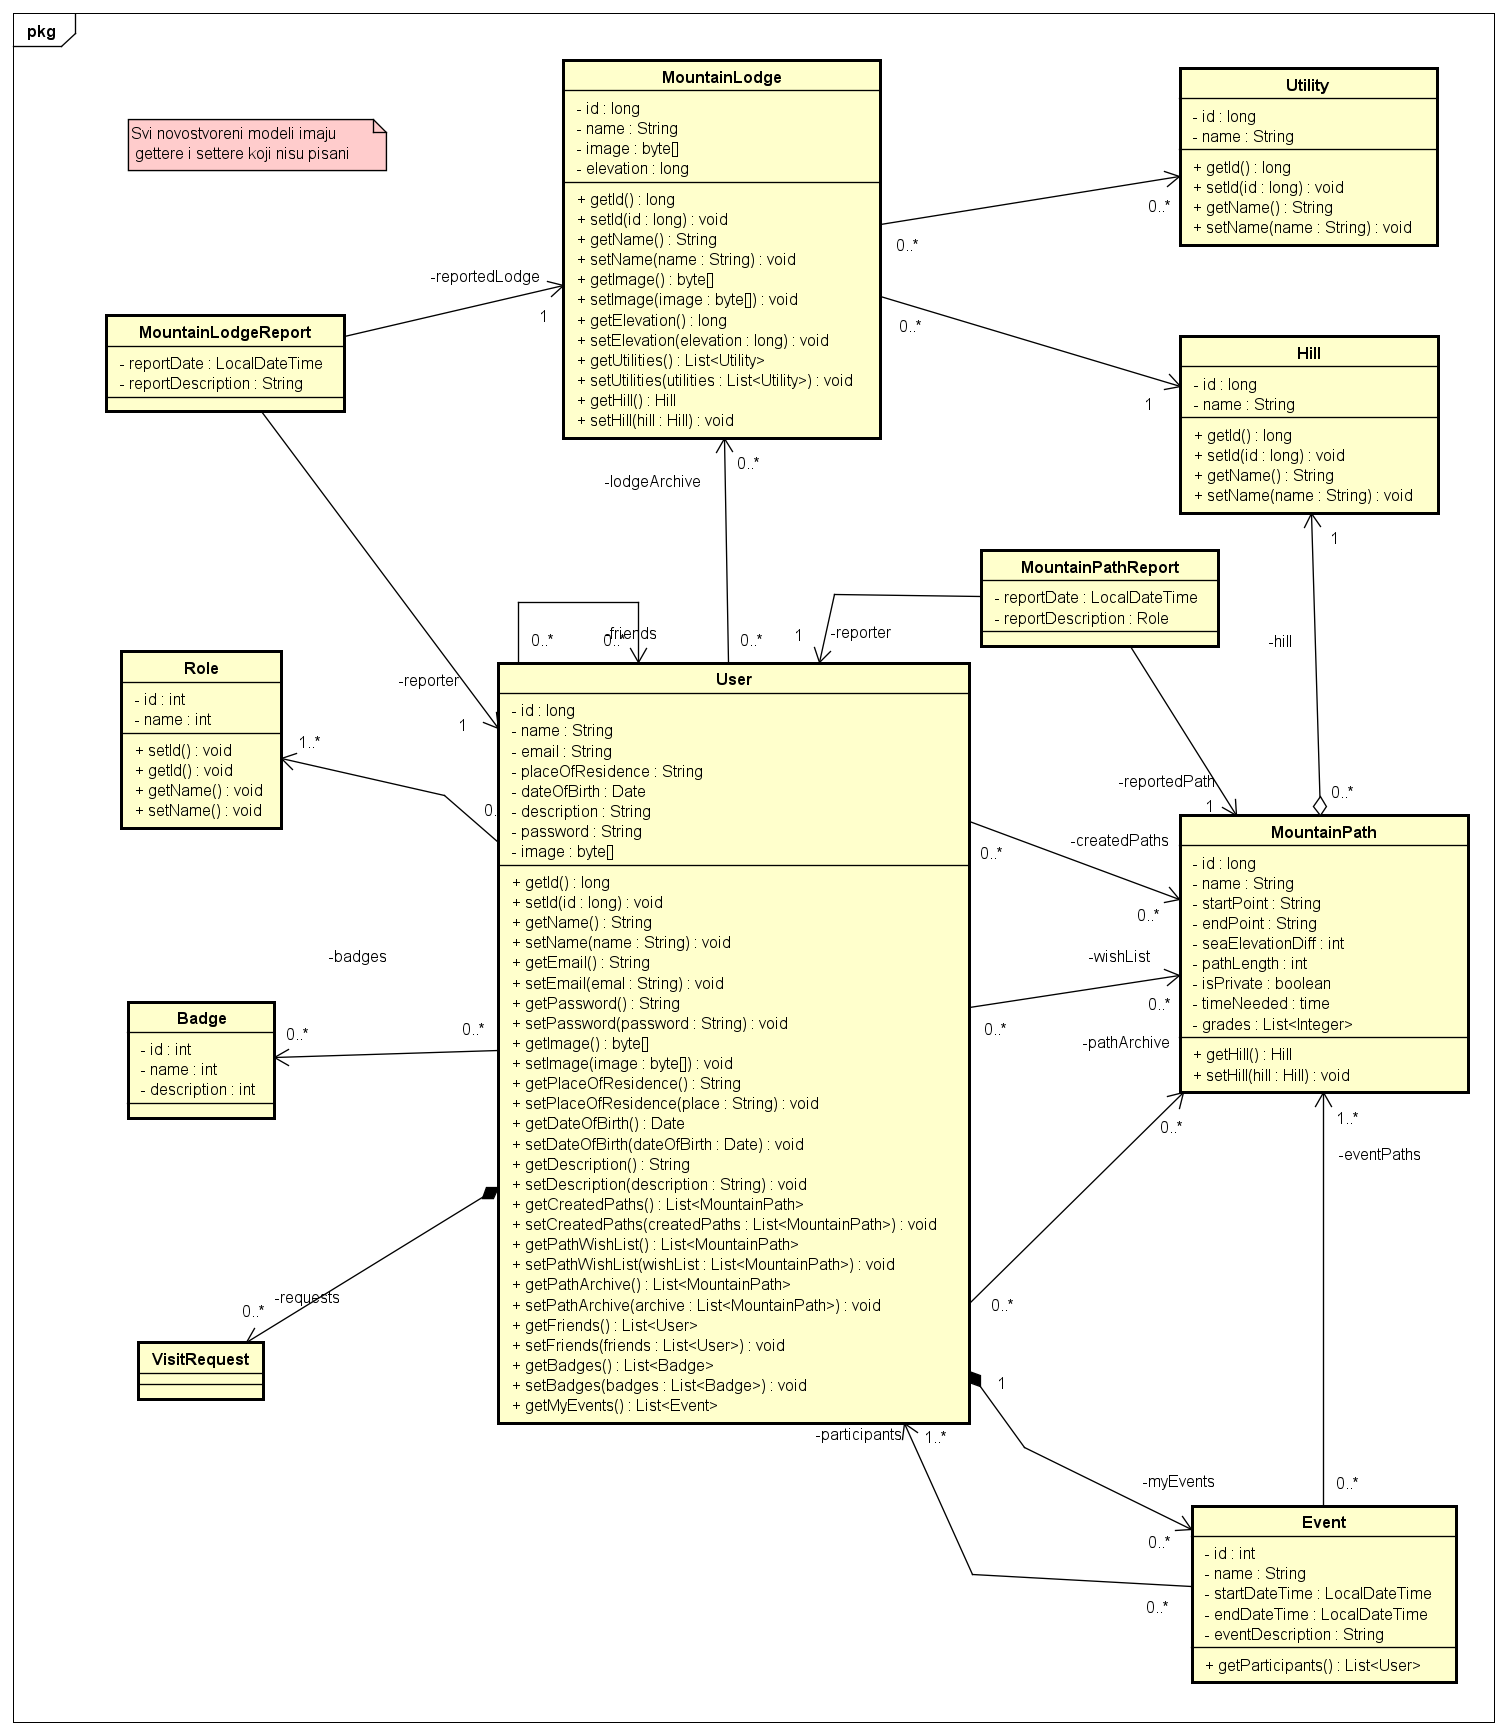
\includegraphics[scale=0.6, height=170mm, width=165mm]{dijagrami/future-model.png} %veličina slike u odnosu na originalnu datoteku i pozicija slike
				\centering
				\caption{Dijagram razreda - idejna razrada daljnjih modela}
				\label{fig:dijagrami_razreda3}
			\end{figure}
			\newpage
			\subsubsection{Sloj nadglednik - servis - repozitorij}
			Ovaj sloj predstavlja sve operacije koje naš sustav obavlja. Razrađen je po oblikovnom obrascu "MVC". Zapravo se ovaj sloj sastoji od tri podsloja, a to su: 
			\begin{itemize}
				\item 
					Sloj repozitorija - metode pristupa bazi podataka, dohvat modela
				\item
					Sloj servisa - tu se obavlja sva naša poslovna logika, pozivaju se metode repozitorija dohvaćaju se podaci
				\item Sloj nadglednika - prima zahtjeve od korisnika i poziva metoda servisnog sloja	
			\end{itemize}
			Razredi koji su trenutno implementirani u ovom sloju prikazani su na dijagramu slijedno, od najnižeg podsloja odnosno pristupa bazi podataka pa sve do podsloja nadglednika koji prima i delegira zahtjeve korisnika.
			Dijagram se sastoji od nekoliko nadglednika: \textit{MountainLodgeController}, \textit{HillController} te \textit{UserController}, a svi su označeni anotacijom \textit{@RestController}. 
			
			Podsloj nadglednika povezan je sa servisnim slojem preko konkretnog primjerka razreda servisnog sloja kojeg čine razredi \textit{MountainLodgeQueryServiceImpl}, \textit{HillQueryServiceImpl} te \textit{UserQueryServiceImpl}, a oni predstavljaju implementacije odgovarajućih servisnih sučelja koji su također označeni na dijagramu.
			
			 Naposljetku, servisni sloj povezan je sa slojem repozitorija preko sučelja konkretnog repozitorija relevantnog za taj servis. U našem slučaju to su sučelja: \textit{MountainLodgeRepository}, \textit{HillRepository} te \textit{UserRepository}. Svako sučelje repozitorija nasljeđuje sučelje \textit{JpaRepository} koje sadrži konkretnu implementaciju upita nad bazom podataka.
			 
			  Sučelje \textit{JpaSpecificationExecutor} omogućuje nam korištenje specifikacije \textit{MountainLodgeSearchSpecification} prilikom pretraživanja planinarskih domova iz baze podataka.
			\begin{figure}[H]
				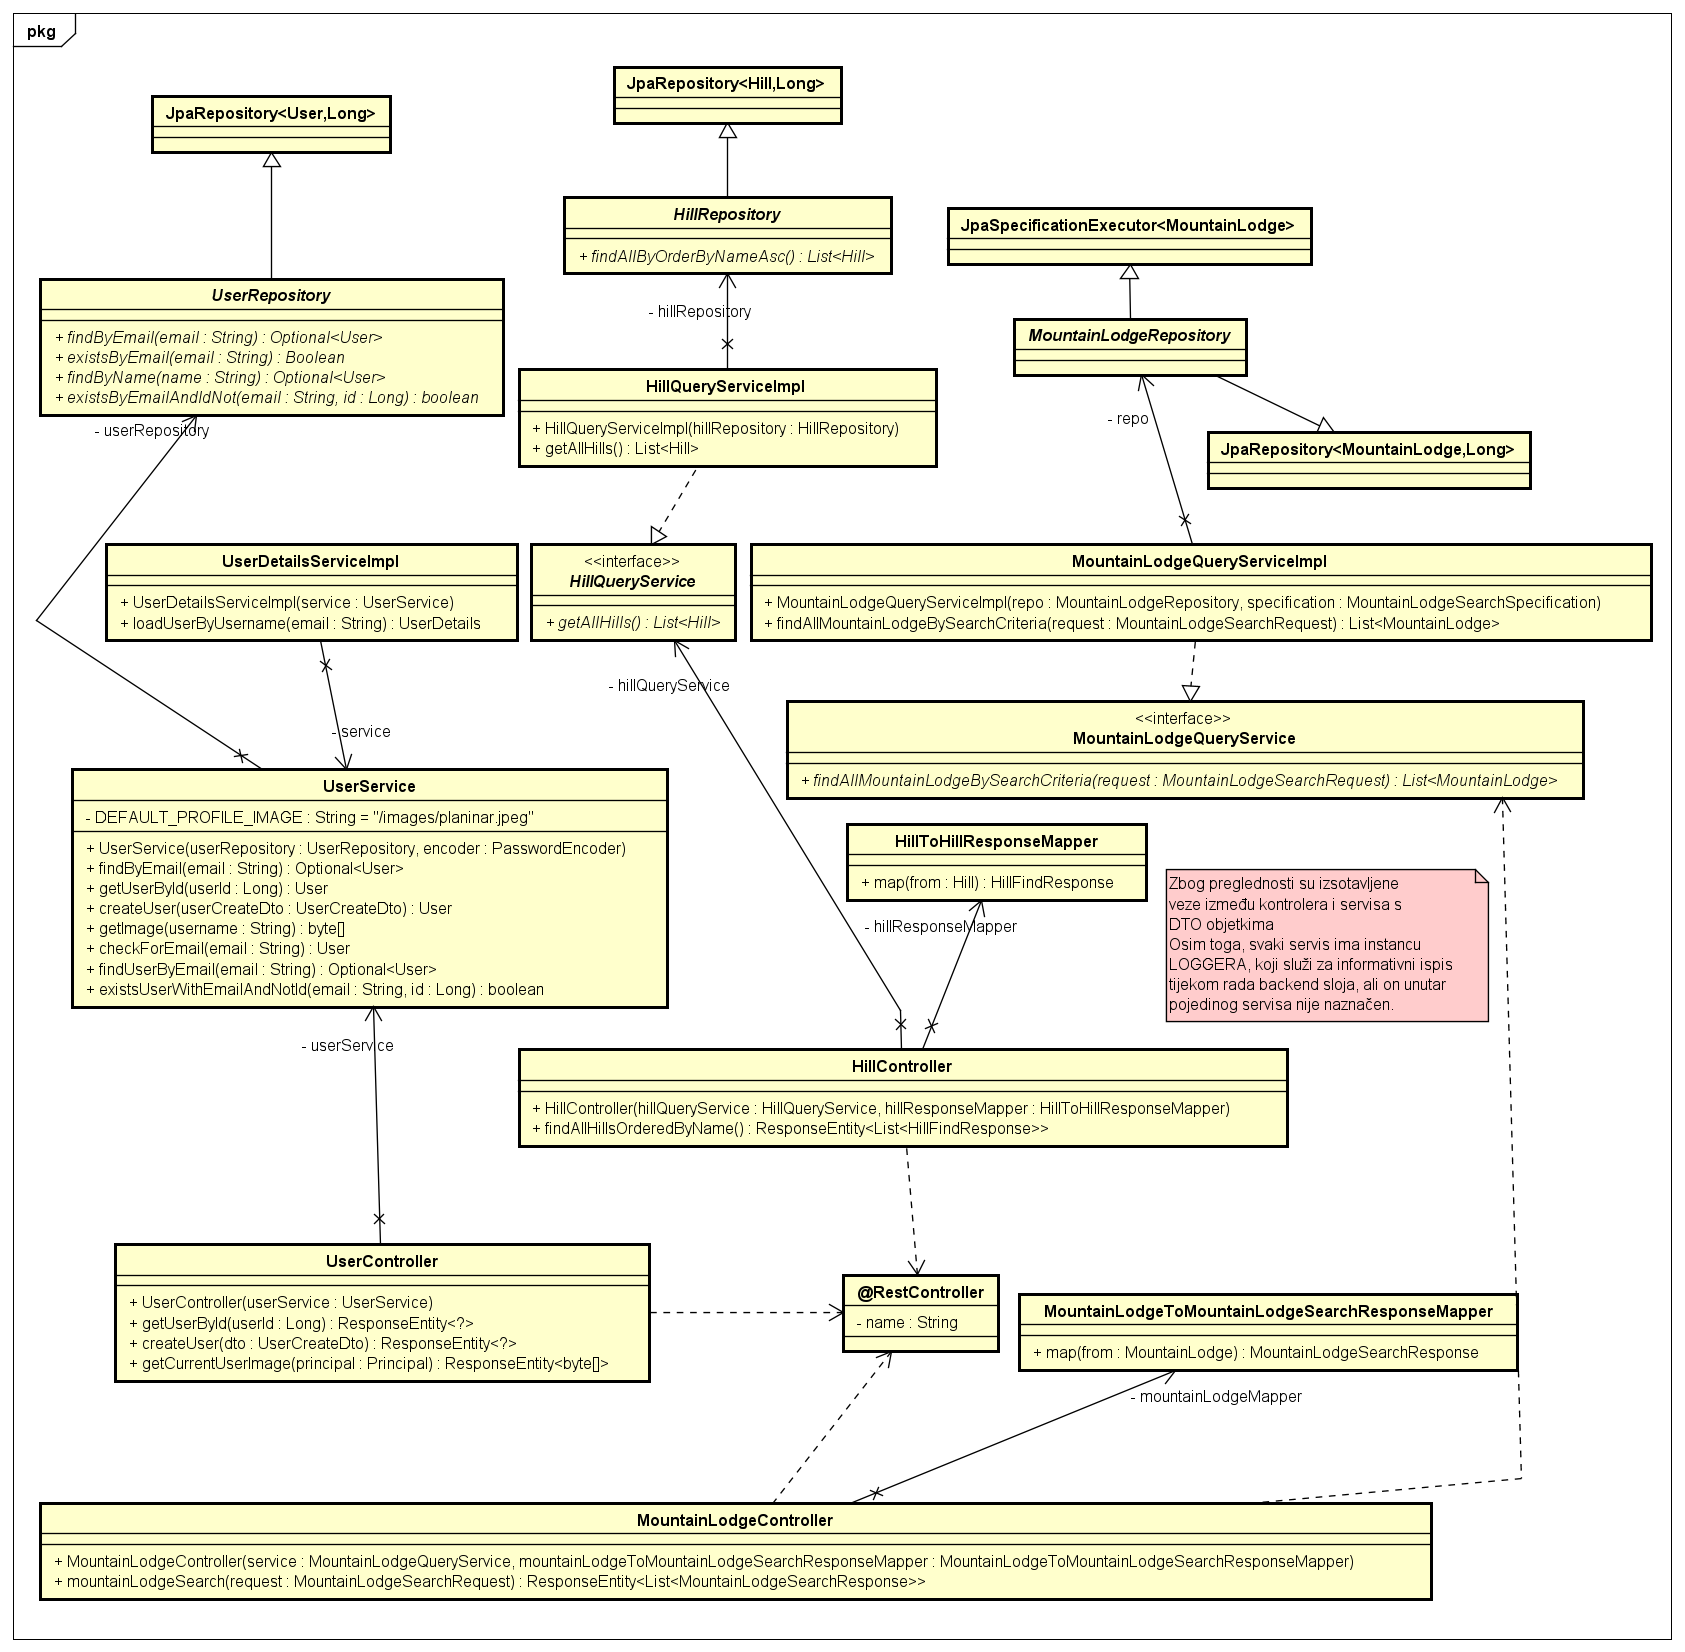
\includegraphics[scale=0.6, height=175mm, width=165mm]{dijagrami/rest.png} %veličina slike u odnosu na originalnu datoteku i pozicija slike
				\centering
				\caption{Dijagram razreda - sloj nadglednik - servis - repozitorij}
				\label{fig:dijagrami_razreda4}
			\end{figure}
			\newpage
			\subsubsection{Razredi vezani uz sigurnost i pomoćni razredi}
			Prilikom prijave korisnika, zahtjev za prijavu se šalje na back end, točnije do nadglednika. Zahtjev se provjerava u razredu \textit{JWTAuthenticationFilter} pomoću metode \textit{attemptAuthentication} koja stvara instancu razreda \textit{UserLogin} i šalje ga na provjeru.
			 
			 Provjera se vrši tako da se zove metoda \textit{loadUserByUsername} razreda \textit{UserDetailsServiceImpl}, a ona provjerava postoji li korisnik koji sadrži e-mail koji je poslan unutar zahtjeva. 
			 
			 Nakon utvrđivanja da ta osoba postoji \textit{Spring security modul} provjerava lozinku i druge podatke vezane uz prijavu. Nakon uspješne prijave pomoću metode \textit{successfulAuthentication} se generira jedinstveni token (identifikator) i šalje korisniku. Svojstva tokena poput trajanja se određuju u razredu \textit{SecurityConstants}. 
			
			Prijavljeni korisnik za vrijeme rada unutar Web aplikacije svaki zahtjev obavlja pomoću jedinstvenog tokena koji mu je dodijeljen, a koji se provjerava unutar razreda \textit{JWTAuthorizationFilter}. 
			
			Metoda \textit{getPasswordEncoder} razreda \textit{Configuration} služi da bi definirali enkoder za zaštitu lozinki. 
			
			Razred \textit{UniqueEmailValidator} prilikom registracije provjerava postoji li u bazi podataka korisnik kojem je e-mail isti e-mailu zahtjeva. Budući da ne možemo imati dva korisnika s istom adresom elektroničke pošte, u tom slučaju događa se iznimka \textit{UserWithEmailExistsException}.  
			
			Razredi \textit{NoImageException} i \textit{ResourceNotFoundException} modeliraju iznimke koje se mogu dogoditi prilikom rada sustava.
			Razred \textit{MountainLodgeSearchSpecification} koji je konkretna implementacija parametriziranog sučelja \textit{BaseSpecification} omogućava nam pretraživanje planinarskih domova prema određenim kriterijima.
			
		
			\begin{figure}[H]
				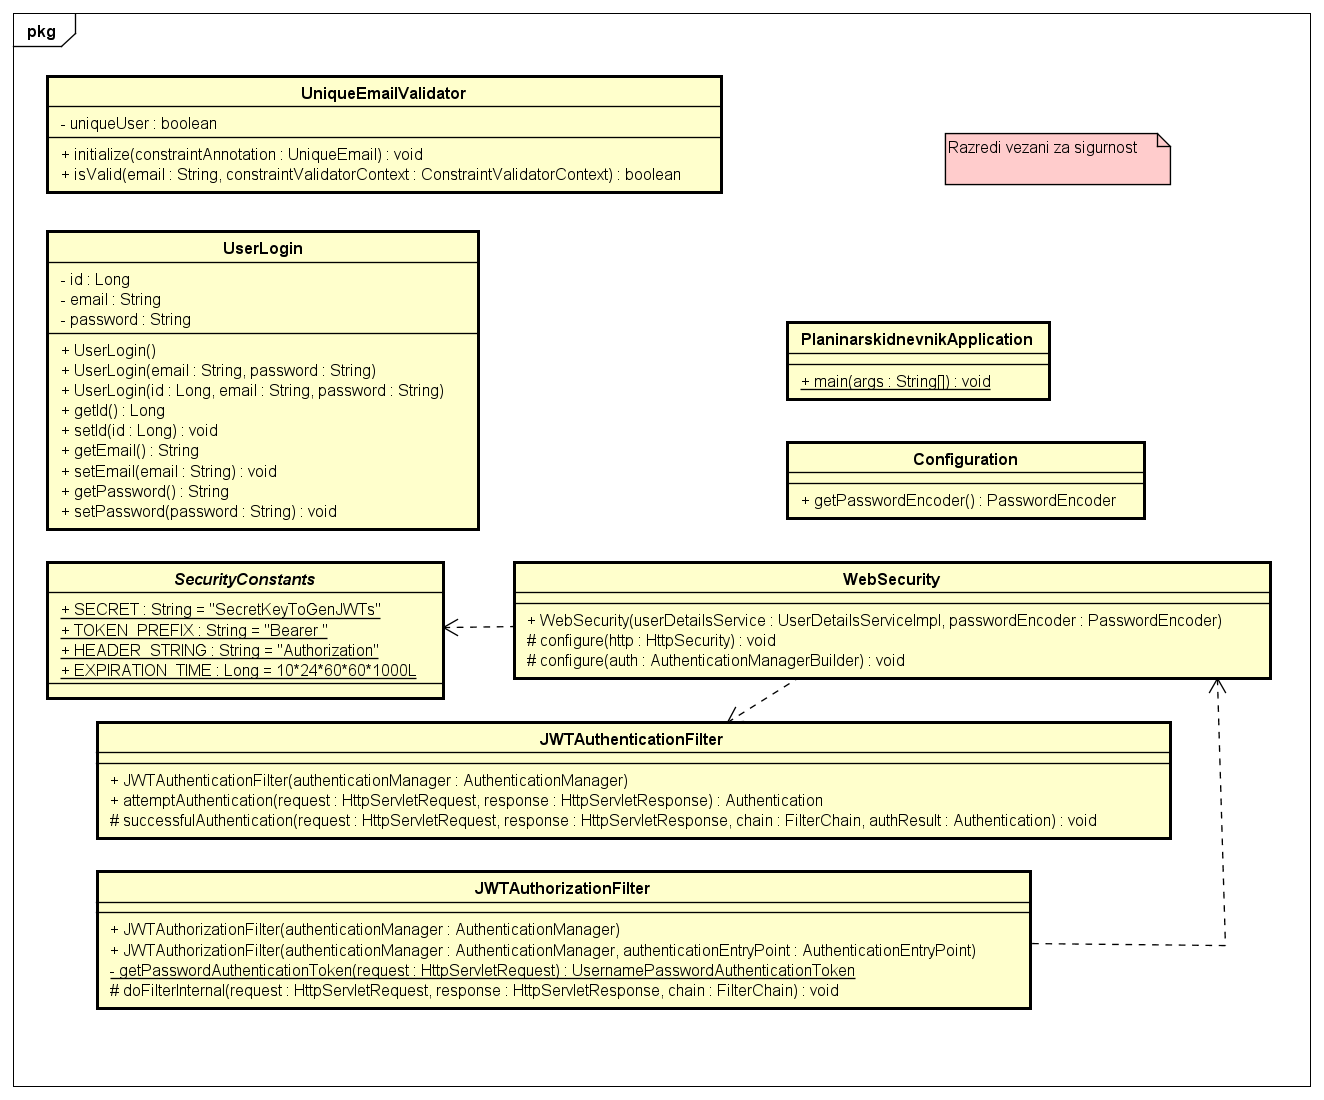
\includegraphics[scale=0.6, height=175mm, width=165mm]{dijagrami/helpers-class.png} %veličina slike u odnosu na originalnu datoteku i pozicija slike
				\centering
				\caption{Dijagram razreda - sigurnost i pomoćne metode}
				\label{fig:dijagrami_razreda5}
			\end{figure}
			
			\eject
			
			
			
			
			\eject
		
		%\section{Dijagram stanja}
			
			
		%	\textbf{\textit{dio 2. revizije}}\\
		%	
		%	\textit{Potrebno je priložiti dijagram stanja i opisati ga. Dovoljan je jedan dijagram stanja koji prikazuje \textbf{značajan dio funkcionalnosti} sustava. Na primjer, stanja korisničkog sučelja i tijek korištenja neke ključne funkcionalnosti jesu značajan dio sustava, a registracija i prijava nisu. }
			
			
		%	\eject 
		
		%\section{Dijagram aktivnosti}
		%	
		%	\textbf{\textit{dio 2. revizije}}\\
			
		%	 \textit{Potrebno je priložiti dijagram aktivnosti s pripadajućim opisom. Dijagram aktivnosti treba prikazivati značajan dio sustava.}
			
		%	\eject
		%\section{Dijagram komponenti}
		
		%	\textbf{\textit{dio 2. revizije}}\\
		
		%	 \textit{Potrebno je priložiti dijagram komponenti s pripadajućim opisom. Dijagram komponenti treba prikazivati strukturu cijele aplikacije.}
			\section{Dijagram komponenti}
		Dijagrami komponenti prikazuju komponente sustava i njihove međusobne odnose. Komponenta je fizička i stvarna implementacija logičkih elemenata sustava, npr. razreda i sučelja. Često se kaže sa su u UML-u sve fizičke "stvari" modelirane kao komponente. Sustavu pristupamo preko dva različita sučelja. Preko jednog dohvaćamo HTML, CSS I TSX datoteke, pomoću kojih poslužujemo datoteke koje pripadaju front end-u aplikacije, a preko drugog sučelja dohvaćamo JSON podatke kojima pristupamo preko REST API komponente, a pomoću nje poslužujemo datoteke koje pripadaju back end-u aplikacije. Frontend sadrži komponentu Router koja pomoću zatraženog url-a na sučelje poslužuje odgovarajuću datoteku. Također sadrži i niz TypeScript datoteka koje su podijeljene u logičke cjeline, a naziv im je dodijeljen po tipu aktora koji pristupaju tim datotekama. React biblioteka je temeljna za sve TypeScript datoteke jer se preko nje dohvaćaju gotove komponente koje su ključne za prikaz podataka, primjerice gumbi i forme. Za dohvat podataka iz baze podataka pomoću SQL upita zadužen je Jdbc framework. Kada se podaci dohvate iz baze, šalju se MVC arhitekturi u obliku DTO. Aplikacija Planinarski dnevnik preko gore navedenih sučelja komunicira sa Reactovim komponentama i ovisno o korisnikovim željama prikazuje i dohvaća zatražene datoteke.
		
		\begin{figure}[H]
			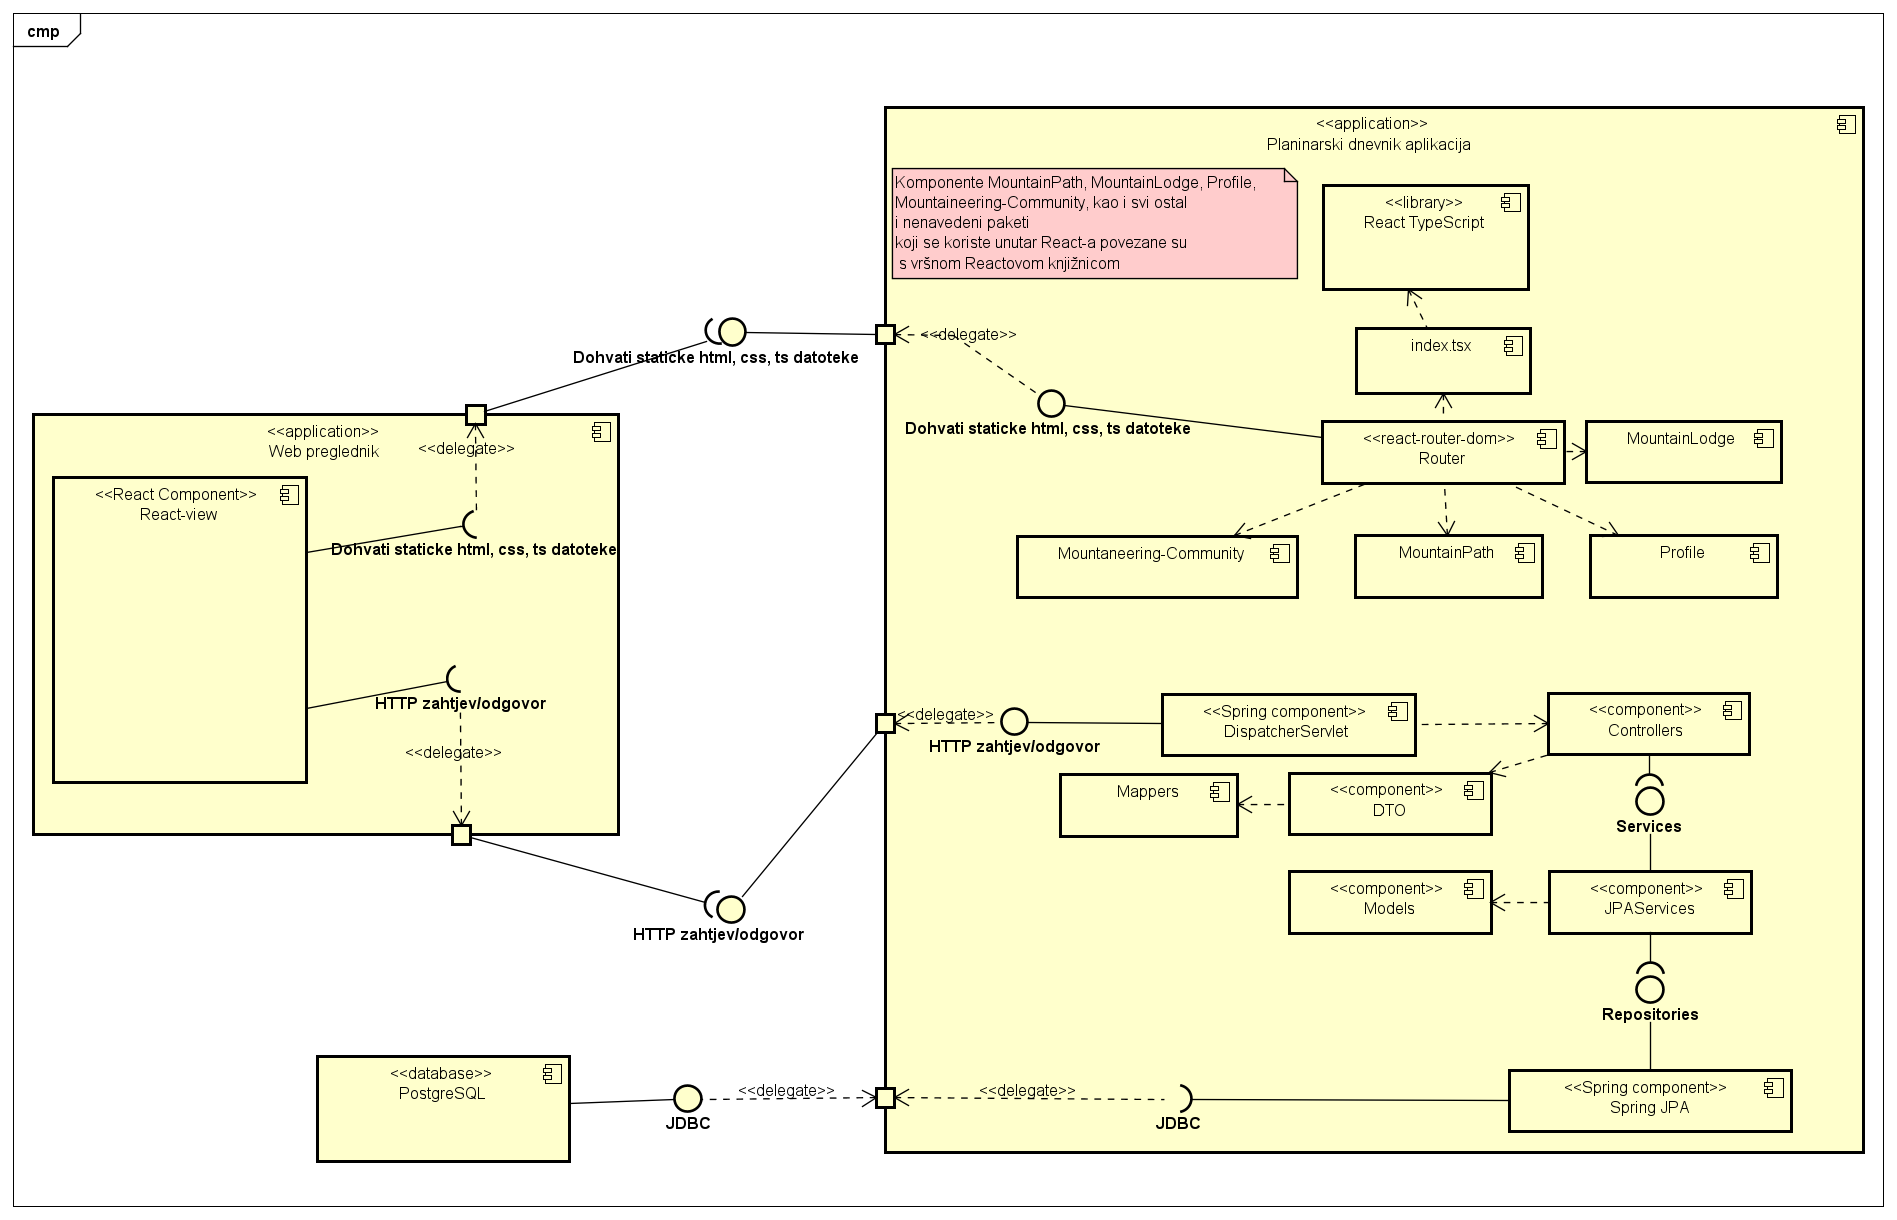
\includegraphics[scale=0.4, height=170mm, width=165mm]{dijagrami/dijagram-komponenti.png} %veličina slike u odnosu na originalnu datoteku i pozicija slike
			\centering
			\caption{Dijagram komponenti}
			\label{fig:dijagrami-komponenti.png}
		\end{figure}
		
		\eject
	\chapter{Implementacija i korisničko sučelje}
		
		
		\section{Korištene tehnologije i alati}
		
			\textbf{\textit{dio 2. revizije}}
			
			 \textit{Detaljno navesti sve tehnologije i alate koji su primijenjeni pri izradi dokumentacije i aplikacije. Ukratko ih opisati, te navesti njihovo značenje i mjesto primjene. Za svaki navedeni alat i tehnologiju je potrebno \textbf{navesti internet poveznicu} gdje se mogu preuzeti ili više saznati o njima}.
			 		
			\eject 
		
	
		\section{Ispitivanje programskog rješenja}
			
			\subsection{Ispitivanje komponenti}
			\textit{Potrebno je provesti ispitivanje jedinica (engl. unit testing) nad razredima koji implementiraju temeljne funkcionalnosti. Razraditi \textbf{minimalno 6 ispitnih slučajeva} u kojima će se ispitati redovni slučajevi, rubni uvjeti te izazivanje pogreške (engl. exception throwing). Poželjno je stvoriti i ispitni slučaj koji koristi funkcionalnosti koje nisu implementirane. Potrebno je priložiti izvorni kôd svih ispitnih slučajeva te prikaz rezultata izvođenja ispita u razvojnom okruženju (prolaz/pad ispita). }
			
			
			
			\subsection{Ispitivanje sustava}
			
			  Ispitivanje smo proveli koristeći Selenium WebDriver unutar JUnit testova. Cilj ispitivanje bio je provjera nekih glavnih funkcionalnosti sustava i pronalazak pogrešaka. WebDriver potrebno je instalirati lokalno na računalo i prilikom pokretanja postaviti putanju koja se nalazi u varijablama okruženja sustava. Prilikom testiranja aplikacija se pokretala na lokalnom računalu zato što je Heroku servis na kojemu je aplikacija puštena u pogon dosta sporiji, pa bi testovi trajali nešto dulje vremena.
			  Slika testova koji su se uspješno izvršili i na aplikaciji puštenoj u pogon na servisu Heroku će biti priložena.\\
	
		 	\textbf{\textit{Ispitni slučaj 1: Prijava planinara u sustav s ispravnim/neispravnim podacima}}
		 	
		 	\begin{lstlisting}
		 	public void testLoginBadAndGoodCreds() throws InterruptedException {
		 		//Driver setup...
		 		System.setProperty("webdriver.chrome.driver", "/path...");
		 		WebDriver driver = new ChromeDriver(); 
		 		driver.manage().timeouts().implicitlyWait(Duration.of(20, ChronoUnit.SECONDS));
		 		
		 		driver.get("http://localhost:3000/home");
		 		WebElement loginButton = driver.findElement(By.id("log-button"));
		 		loginButton.click();
		 		String loginUrl = driver.getCurrentUrl();
		 		assertTrue(loginUrl.contains("/login"));
		 		WebElement Emailelement = driver.findElement(By.id("email"));        
		 		Emailelement.sendKeys("luka.ravenscak");   
		 		WebElement passElement = driver.findElement(By.id("password"));
		 		passElement.sendKeys("password");
		 		driver.findElement(By.className("submitButton")).click();
		 		WebElement element = driver.findElement(By.className("errorText"));
		 		assertEquals("Neispravan oblik mail-a.", element.getText());
		 		Emailelement.clear();
		 		Emailelement.sendKeys("luka.ravenscak@fer.hr");
		 		passElement.clear();
		 		passElement.sendKeys("mypassword");
		 		driver.findElement(By.className("submitButton")).click();
		 		element = driver.findElement(By.id("error-span"));
		 		assertEquals("Neispravan e-mail ili lozinka.", element.getText());
		 		passElement.clear();
		 		passElement.sendKeys("password");
		 		driver.findElement(By.className("submitButton")).click();
		 		Thread.sleep(1000);
		 		assertTrue(driver.getCurrentUrl().contains("/mountaineering-community"));
		 		
		 		driver.quit();
		 	}
		 	\end{lstlisting}
	 	
	 	 U 1. ispitnom slučaju ispitana je funkcionalnost prijave u sustav. Prvo se dohvati početna stranica aplikacije te se odabire opcija "Prijavi se" koja se nalazi na zaglavlju stranice. Zatim se unese neispravni oblik email-a, na što aplikacija vraća obavijest "Neispravan oblik mail-a.", nakon toga se unose valjani email i neispravna lozinka, aplikacija reagira tako da vrati obavijest "Neispravan e-mail ili lozinka.". Na kraju se unesu ispravni podaci za prijavu i aplikacija reagira uspješnom prijavnom korisnika u sustav i odvede korisnika na stranicu vlastite planinarske zajednice.\newline
	 	 
	 		\textbf{\textit{Ispitni slučaj 2: Planinar pretražuje ostale korisnike}}
	 	
	 	\begin{lstlisting}
	 		public void testSearchAdminOnAllUserSearchPage() throws InterruptedException {
	 			
	 			//Driver setup
	 			driver.get("http://localhost:3000/login");
	 			
	 			WebElement element = driver.findElement(By.id("email"));        
	 			element.sendKeys("luka.ravenscak@fer.hr");
	 			element = driver.findElement(By.id("password"));
	 			element.sendKeys("password");
	 			driver.findElement(By.className("submitButton")).click();
	 			Thread.sleep(2000);
	 			assertTrue(driver.getCurrentUrl().contains("/mountaineering-community"));
	 			
	 			WebElement searchAllButton = driver.findElement(By.className("search-all-button"));
	 			searchAllButton.click(); 
	 			
	 			assertTrue(driver.getCurrentUrl().contains("/users/search"));    
	 			element = driver.findElement(By.name("searchText"));        
	 			element.sendKeys("admin");
	 			driver.findElement(By.name("searchText")).click();
	 			driver.findElement(By.className("all-user-photo")).click();
	 			Thread.sleep(2000);	    
	 			assertTrue(driver.getCurrentUrl().contains("/profile"));
	 			
	 			assertEquals("admin", driver.findElement(By.id("name-profile")).getAttribute("value"));
	 			driver.quit();
	 		}
	 	\end{lstlisting}
 	
	 	U 2. ispitnom slučaju ispitana je funkcionalnost pretrage svih korisnika od strane planinara. Prvo se provede prijava planinara u sustav, zatim prijavljeni korisnik odabire opciju "Pretraži sve planinare" te ga aplikacija preusmjeri na stranicu za pretragu svih korisnika. Korisnik u prostor za unos teksta za pretragu upiše "admin" i odabire opciju pretrage, aplikacija u rezultatima pretrage vrati traženog korisnika. Nakon toga korisnik odabere adminovu sličicu profila i aplikacija mu prikaže adminov profil. Testiranje je provedeno na način da se pretražuje profil admina, koji unutar aplikacije uvijek postoji.\newline
	 	
 		\textbf{\textit{Ispitni slučaj 3: Pretraga i arhiviranje posjećenog planinarskog doma}}
 		
 		\begin{lstlisting}
 			public void testMountainLodgeSearchArchiveAndBadgeAdd() throws InterruptedException {
 			//Driver setup
 			
 			driver.get("http://localhost:3000");
 			driver.findElement(By.className("domovi")).click();
 			assertTrue(driver.getCurrentUrl().contains("/mountain-lodge/search"));
 			driver.findElement(By.className("input-search")).sendKeys("Planinarski dom Glavica");	    
 			driver.findElement(By.className("search-button")).click();
 			assertEquals("Planinarski dom Glavica", driver.findElement(By.className("mountain-lodge-name")).getText());
 			assertThrows(NoSuchElementException.class, new ThrowingRunnable() {
 				public void run() throws Throwable {
 					driver.findElement(By.className("archive-button-lodge"));
 				}
 			});
 			
 			WebElement loginButton = driver.findElement(By.id("log-button"));
 			loginButton.click();
 			String loginUrl = driver.getCurrentUrl();
 			assertTrue(loginUrl.contains("/login"));
 			WebElement Emailelement = driver.findElement(By.id("email"));        
 			Emailelement.sendKeys("luka.ravenscak@fer.hr");   
 			WebElement passElement = driver.findElement(By.id("password"));
 			passElement.sendKeys("password");
 			driver.findElement(By.className("submitButton")).click();
 			Thread.sleep(2000);
 			assertTrue(driver.getCurrentUrl().contains("/mountaineering-community"));
 			driver.findElement(By.className("logo-image")).click();
 			
 			driver.findElement(By.className("domovi")).click();
 			assertTrue(driver.getCurrentUrl().contains("/mountain-lodge/search"));
 			driver.findElement(By.className("input-search")).sendKeys("Planinarski dom Glavica");	    
 			driver.findElement(By.className("search-button")).click();
 			assertEquals("Planinarski dom Glavica", driver.findElement(By.className("mountain-lodge-name")).getText());
 			
 			WebElement archiveButton = driver.findElement(By.className("archive-button-lodge"));
 			assertEquals("ARHIVIRAJ",driver.findElement(By.className("MuiButton-label"))
 			.getText());
 			archiveButton.click();
 			Thread.sleep(3000);
 			assertEquals("ARHIVIRANO",driver.findElement(By.className("MuiButton-label"))
 			.getText());
 			
 			driver.findElement(By.className("profil-image")).click();
 			driver.findElement(By.id("my-profile")).click();
 			String badgeDesc = driver.findElement(By.className("badge-image")).getAttribute("title");
 			assertEquals("Imam barem 1 posjećen planinarski dom!", badgeDesc);
 			
 			driver.quit();
 		}
 		\end{lstlisting}
 	
 		U 3. ispitnom slučaju ispitana je funkcionalnost pretraživanja i arhiviranja planinarskog doma, te je testirano da pristup arhiviranju imaju samo prijavljeni korisnici. Neprijavljen korisnik odabire opciju "Pretraga planinarskih domova", u prostor za unos teksta upisuje "Planinarski dom Glavica". Taj dom postoji u bazi podataka i aplikacija mu kao rezultat pretrage prikaže traženi planinarski dom. Zatim se testira da aplikacija neprijavljenom korisniku ne nudi mogućnost arhiviranja doma. Nakon što je taj dio testa aplikacija zadovoljen, test se nastavlja i korisnik se prijavi u sustav kao planinar te ponavlja istu radnju. Ovaj put aplikacija mu prikazuje traženi dom, ali korisnik ima mogućnost arhiviranja doma. Korisnik odabire opciju "Arhiviraj", aplikacija na tu akciju mijenja opis uz navedeni dom u "Arhivirano", te odabrani dom sprema u popis posjećenih domova planinara koji je odabrao opciju "Arhiviraj". Korisnik odabire opciju "Moj profil", aplikacija mu prikaže profil na kojem se može vidjeti priznanje (bedž) kojeg je dobio posjetom jednog planinarskog doma, uz opis postignuća "Imam barem 1 posjećen planinarski dom!"\newline
 		
 		 	\textbf{\textit{Ispitni slučaj 4: Slanje zahtjeva za prijateljstvo i primitak obavijesti o prihvaćenom zahtjevu}}
 		
 		\begin{lstlisting}
 			public void testAddFriendAndFriendRequestApproveOrDeclineAndFriendNotification() throws InterruptedException {
 				//Driver setup
 				
 				driver.get("http://localhost:3000/login");      
 				driver.findElement(By.id("email")).sendKeys("luka.ravenscak@fer.hr");   
 				driver.findElement(By.id("password")).sendKeys("password");
 				driver.findElement(By.className("submitButton")).click();
 				Thread.sleep(2000);
 				
 				WebElement searchAllButton = driver.findElement(By.className("search-all-button"));
 				searchAllButton.click(); 
 				assertTrue(driver.getCurrentUrl().contains("/users/search"));
 				WebElement element = driver.findElement(By.name("searchText"));        
 				element.sendKeys("admin");
 				driver.findElement(By.name("searchText")).click();
 				driver.findElement(By.className("all-user-photo")).click();
 				Thread.sleep(2000);	    
 				assertTrue(driver.getCurrentUrl().contains("/profile"));
 				
 				driver.findElement(By.className("button-profile")).click();
 				assertTrue(driver.findElement(By.className("button-profile-fr"))
 				.getText().contains("Zahtjev poslan"));
 				driver.findElement(By.className("profil-image")).click();
 				driver.findElement(By.id("logout-b")).click();
 				Thread.sleep(2000);
 				driver.findElement(By.id("log-button")).click();
 				driver.findElement(By.id("email")).sendKeys("admin@fer.hr");   
 				driver.findElement(By.id("password")).sendKeys("password");
 				driver.findElement(By.className("submitButton")).click();
 				Thread.sleep(2000);
 				driver.findElement(By.className("profil-image")).click();
 				driver.findElement(By.id("fr-requests")).click();
 				assertEquals("Luka Ravenscak", driver.findElement(By.className("user-name")).getText());
 				driver.findElement(By.className("submitButtonaccept")).click();
 				
 				driver.findElement(By.className("profil-image")).click();
 				driver.findElement(By.id("logout-b")).click();
 				Thread.sleep(2000);
 				driver.findElement(By.id("log-button")).click();
 				driver.findElement(By.id("email")).sendKeys("luka.ravenscak@fer.hr");   
 				driver.findElement(By.id("password")).sendKeys("password");
 				driver.findElement(By.className("submitButton")).click();
 				Thread.sleep(2000);
 				driver.findElement(By.className("profil-image")).click();
 				driver.findElement(By.id("fr-notifications")).click();
 				assertTrue(driver.findElement(By.className("user-name-span"))
 				.getText().contains("Postali ste prijatelj s"));
 				assertTrue(driver.findElement(By.className("user-name"))
 				.getText().contains("admin"));
 				driver.quit();
 			}
 		\end{lstlisting}
 	
 		U 4. ispitnom slučaju ispitana je funkcionalnost slanja zahtjeva za prijateljstvo i primanje obavijesti o prihvaćenom zahtjevu. Prvo se korisnik prijavi kao "luka.ravenscak@fer.hr" te provede radnje kao u testu 2. Dolaskom na adminov profil odabere opciju "Dodaj prijatelja". Aplikacija promijeni status gumba u "Zahtjev poslan" te proslijedi zahtjev za prijateljstvo adminu. Zatim se korisnik odjavi, te odlazimo na profil admina, nakon čega korisnik provjeri zahtjeve za prijateljstvo i prihvati zahtjev korisnika "luka.ravenscak@fer.hr".
 		Nakon što je admin uspješno prihvatio zahtjev korisnik se odjavi i prijavi ponovno kao "luka.ravenscak@fer.hr". Nakon toga aplikacija će korisniku "luka.ravenscak@fer.hr" prikazati novu obavijest o prihvaćenom zahtjevu za prijateljstvo od strane admina. 
 		
		
		\begin{figure}[H]
			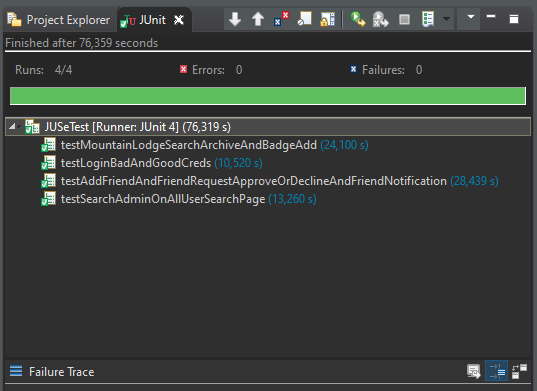
\includegraphics[scale=0.6, height=65mm, width=100mm]{slike/test_results.png} %veličina slike u odnosu na originalnu datoteku i pozicija slike
			\centering
			\caption{Uspješno izvršeni Selenium testovi - lokalno računalo}
			\label{fig:test_results}
		\end{figure}
		
			\eject 
		
		
		\section{Dijagram razmještaja}
			
			\textbf{\textit{dio 2. revizije}}
			
			 \textit{Potrebno je umetnuti \textbf{specifikacijski} dijagram razmještaja i opisati ga. Moguće je umjesto specifikacijskog dijagrama razmještaja umetnuti dijagram razmještaja instanci, pod uvjetom da taj dijagram bolje opisuje neki važniji dio sustava.}
			
			\eject 
		
		\section{Upute za puštanje u pogon}
		
			\textbf{\textit{dio 2. revizije}}\\
		
			 \textit{U ovom poglavlju potrebno je dati upute za puštanje u pogon (engl. deployment) ostvarene aplikacije. Na primjer, za web aplikacije, opisati postupak kojim se od izvornog kôda dolazi do potpuno postavljene baze podataka i poslužitelja koji odgovara na upite korisnika. Za mobilnu aplikaciju, postupak kojim se aplikacija izgradi, te postavi na neku od trgovina. Za stolnu (engl. desktop) aplikaciju, postupak kojim se aplikacija instalira na računalo. Ukoliko mobilne i stolne aplikacije komuniciraju s poslužiteljem i/ili bazom podataka, opisati i postupak njihovog postavljanja. Pri izradi uputa preporučuje se \textbf{naglasiti korake instalacije uporabom natuknica} te koristiti što je više moguće \textbf{slike ekrana} (engl. screenshots) kako bi upute bile jasne i jednostavne za slijediti.}
			
			
			 \textit{Dovršenu aplikaciju potrebno je pokrenuti na javno dostupnom poslužitelju. Studentima se preporuča korištenje neke od sljedećih besplatnih usluga: \href{https://aws.amazon.com/}{Amazon AWS}, \href{https://azure.microsoft.com/en-us/}{Microsoft Azure} ili \href{https://www.heroku.com/}{Heroku}. Mobilne aplikacije trebaju biti objavljene na F-Droid, Google Play ili Amazon App trgovini.}
			
			
			\eject 
	\chapter{Zaključak i budući rad}
		
		\textbf{\textit{dio 2. revizije}}\\
		
		 \textit{U ovom poglavlju potrebno je napisati osvrt na vrijeme izrade projektnog zadatka, koji su tehnički izazovi prepoznati, jesu li riješeni ili kako bi mogli biti riješeni, koja su znanja stečena pri izradi projekta, koja bi znanja bila posebno potrebna za brže i kvalitetnije ostvarenje projekta i koje bi bile perspektive za nastavak rada u projektnoj grupi.}
		
		 \textit{Potrebno je točno popisati funkcionalnosti koje nisu implementirane u ostvarenoj aplikaciji.}
		
		\eject 
	\chapter*{Popis literature}
		\addcontentsline{toc}{chapter}{Popis literature}
	 	
		
		\begin{enumerate}
			
			
			\item  Programsko inženjerstvo, FER ZEMRIS, \url{http://www.fer.hr/predmet/proinz}
			
			\item  I. Sommerville, "Software engineering", 8th ed, Addison Wesley, 2007.
			
			\item  T.C.Lethbridge, R.Langaniere, "Object-Oriented Software Engineering", 2nd ed. McGraw-Hill, 2005.
			
			\item  I. Marsic, Software engineering book``, Department of Electrical and Computer Engineering, Rutgers University, \url{http://www.ece.rutgers.edu/~marsic/books/SE}
			
			\item  The Unified Modeling Language, \url{https://www.uml-diagrams.org/}
			
			\item  Astah Community, \url{http://astah.net/editions/uml-new}
		\end{enumerate}
		
		 
	
	
	\begingroup
	\renewcommand*\listfigurename{Indeks slika i dijagrama}
	%\renewcommand*\listtablename{Indeks tablica}
	%\let\clearpage\relax
	\listoffigures
	%\vspace{10mm}
	%\listoftables
	\endgroup
	\addcontentsline{toc}{chapter}{Indeks slika i dijagrama}


	
	\eject 
		
	\chapter*{Dodatak: Prikaz aktivnosti grupe}
		\addcontentsline{toc}{chapter}{Dodatak: Prikaz aktivnosti grupe}
		
		\section*{Dnevnik sastajanja}
		
		\textbf{\textit{Kontinuirano osvježavanje}}\\
		
		 \textit{U ovom dijelu potrebno je redovito osvježavati dnevnik sastajanja prema predlošku.}
		
		\begin{packed_enum}
			\item  sastanak
			
			\item[] \begin{packed_item}
				\item Datum:  7. listopada 2020.
				\item Prisustvovali: I.Martinović, M.Rajnović, N.Kušurin, H.Ladić, L.Ravenšćak, J.Kaselj, D.Konjevod
				\item Teme sastanka: 
				\begin{packed_item}
					\item  Komentiranje zadatka koji smo dobili i komentiranje nejasnih dijelova
					\item  Razgovor o poznavanju tehnologija (Git, Spring, React)
					\item  Dogovor o tutorialima koje treba pogledati na internetu
					\item  Razgovor o funkcioniranju gitlaba
				\end{packed_item}
			\end{packed_item}
			
			\item  sastanak
			\item[] \begin{packed_item}
				\item Datum:  8.listopada 2020.
				\item Prisustvovali: I.Martinović, M.Rajnović, N.Kušurin, H.Ladić, L.Ravenšćak, J.Kaselj, D.Konjevod, K.Labor, M.Bićanić, H.Šimić
				\item Teme sastanka:
				\begin{packed_item}
					\item   Predstavljanje načina rada i uvod u projekt
					\item   Rješavanje nejasnoća vezanih uz zadatak s asistentom i demonstratorom
				\end{packed_item}
			\end{packed_item}
		
			\item  sastanak
			\item[] \begin{packed_item}
				\item Datum:  9.listopada 2020.
				\item Prisustvovali: I.Martinović, M.Rajnović, N.Kušurin, H.Ladić, L.Ravenšćak, J.Kaselj, D.Konjevod
				\item Teme sastanka:
				\begin{packed_item}
					\item   Inicijalizacija projekta (back end i front end) na gitlabu
					\item   Dogovor oko raspodjele poslova vezanih uz dokumentaciju
				\end{packed_item}
			\end{packed_item}
	
			\item sastanak
			\item[] \begin{packed_item}
				\item Datum: 11.listopada 2020.
				\item Prisustvovali: I.Martinović, M.Rajnović, J.Kaselj
				\item Teme sastanka:
				\begin{packed_item}
					\item   Izlučivanje funkcionalnih zahtjeva
				\end{packed_item}
			\end{packed_item}
		
			\item sastanak
			\item[] \begin{packed_item}
				\item Datum: 11.listopada 2020.
				\item Prisustvovali: N.Kušurin, D.Konjevod, H.Ladić
				\item Teme sastanka:
				\begin{packed_item}
					\item   Opis projektnog zadatka
				\end{packed_item}
			\end{packed_item}
		
		\item sastanak
		\item[] \begin{packed_item}
			\item Datum:  15.listopada 2020.
			\item Prisustvovali: N.Kušurin, D.Konjevod, H.Ladić, I.Martinović, M.Rajnović, J.Kaselj, L.Ravenšćak,  K.Labor
			\item Teme sastanka: 
			\begin{packed_item}
				\item   Raspravljanje o funkcionalnim zahtjevima s asistentom
				\item 	Dogovori za buduću komunikaciju
			\end{packed_item}
		\end{packed_item}
	
	\item sastanak
	\item[] \begin{packed_item}
		\item Datum: 15.listopada 2020.
		\item Prisustvovali: N.Kušurin, D.Konjevod, H.Ladić, I.Martinović, M.Rajnović, J.Kaselj, L.Ravenšćak
		\item Teme sastanka: 
		\begin{packed_item}
			\item   Crtanje ekrana
			\item 	Raspodjela daljnjih poslova
		\end{packed_item}
	\end{packed_item}

	\item sastanak
	\item[] \begin{packed_item}
		\item Datum:  19.listopada 2020.
		\item Prisustvovali: N.Kušurin, D.Konjevod
		\item Teme sastanka: 
		\begin{packed_item}
			\item   Scenariji obrazaca uporabe
		\end{packed_item}
	\end{packed_item}
	
	
	\item sastanak
	\item[] \begin{packed_item}
		\item Datum: 20.listopada 2020.
		\item Prisustvovali: I.Martinović, M.Rajnović, L.Ravenšćak
		\item Teme sastanka: 
		\begin{packed_item}
			\item   Modeliranje baze podataka
		\end{packed_item}
	\end{packed_item}
			
			
			\item sastanak
			\item[] \begin{packed_item}
				\item Datum: 22.listopada 2020.
				\item Prisustvovali: I.Martinović, M.Rajnović, L.Ravenšćak, J.Kaselj, H.Ladić, D.Konjevod, N.Kušurin, K.Labor, M.Bićanić
				\item Teme sastanka: 
				\begin{packed_item}
					\item   Pregledavanje dokumentacije i upute za nastavak s asistentom i demosom
				\end{packed_item}
			\end{packed_item}
			
			
			\item sastanak
			\item[] \begin{packed_item}
				\item Datum: 23.listopada 2020.
				\item Prisustvovali: I.Martinović, J.Kaselj, H.Ladić
				\item Teme sastanka: 
				\begin{packed_item}
					\item   Razrada sekvencijskih dijagrama
				\end{packed_item}
			\end{packed_item}
			
			%
			
		\end{packed_enum}
		
		\eject
		\section*{Tablica aktivnosti}
		
			\textbf{\textit{Kontinuirano osvježavanje}}\\
			
			 \textit{Napomena: Doprinose u aktivnostima treba navesti u satima po članovima grupe po aktivnosti.}
					
						
			
			\begin{longtabu} to \textwidth {|X[7, l]|X[1, c]|X[1, c]|X[1, c]|X[1, c]|X[1, c]|X[1, c]|X[1, c]|}
								
				\cline{2-8} \multicolumn{1}{c|}{\textbf{}} &     \multicolumn{1}{c|}{\rotatebox{90}{\textbf{Ivan Martinović }}} & 
				\multicolumn{1}{c|}{\rotatebox{90}{\textbf{Luka Ravenšćak }}} &	\multicolumn{1}{c|}{\rotatebox{90}{\textbf{Marko Rajnović}}} &	\multicolumn{1}{c|}{\rotatebox{90}{\textbf{Josipa Kaselj}}} &
				\multicolumn{1}{c|}{\rotatebox{90}{\textbf{Neda Kušurin}}} &
				\multicolumn{1}{c|}{\rotatebox{90}{\textbf{Helena Ladić}}} &	\multicolumn{1}{c|}{\rotatebox{90}{\textbf{David Konjevod}}} \\ \hline 
				\endfirsthead
				
			
				\cline{2-8} \multicolumn{1}{c|}{\textbf{}} &     \multicolumn{1}{c|}{\rotatebox{90}{\textbf{Ime Prezime voditelja}}} & \multicolumn{1}{c|}{\rotatebox{90}{\textbf{Ime Prezime }}} &	\multicolumn{1}{c|}{\rotatebox{90}{\textbf{Ime Prezime }}} &
				\multicolumn{1}{c|}{\rotatebox{90}{\textbf{Ime Prezime }}} &	\multicolumn{1}{c|}{\rotatebox{90}{\textbf{Ime Prezime }}} &
				\multicolumn{1}{c|}{\rotatebox{90}{\textbf{Ime Prezime }}} &	\multicolumn{1}{c|}{\rotatebox{90}{\textbf{Ime Prezime }}} \\ \hline 
				\endhead
				
				
				\endfoot
							
				 
				\endlastfoot
				
				Upravljanje projektom 		& 7 &  &  &  &  &  & \\ \hline
				Opis projektnog zadatka 	& 3 &  &  &  &  &  & \\ \hline
				
				Funkcionalni zahtjevi       & 7 &  &  &  &  &  &  \\ \hline
				Opis pojedinih obrazaca 	& 8 &  &  &  &  &  &  \\ \hline
				Dijagram obrazaca 			&  &  &  &  &  &  &  \\ \hline
				Sekvencijski dijagrami 		&  &  &  &  &  &  &  \\ \hline
				Opis ostalih zahtjeva 		&  &  &  &  &  &  &  \\ \hline

				Arhitektura i dizajn sustava	 &  &  &  &  &  &  &  \\ \hline
				Baza podataka				& 2 &  &  &  &  &  &   \\ \hline
				Dijagram razreda 			&  &  &  &  &  &  &   \\ \hline
				Dijagram stanja				&  &  &  &  &  &  &  \\ \hline
				Dijagram aktivnosti 		&  &  &  &  &  &  &  \\ \hline
				Dijagram komponenti			&  &  &  &  &  &  &  \\ \hline
				Korištene tehnologije i alati 		&  &  &  &  &  &  &  \\ \hline
				Ispitivanje programskog rješenja 	&  &  &  &  &  &  &  \\ \hline
				Dijagram razmještaja			&  &  &  &  &  &  &  \\ \hline
				Upute za puštanje u pogon 		&  &  &  &  &  &  &  \\ \hline 
				Dnevnik sastajanja 			& 1 &  &  &  &  &  &  \\ \hline
				Zaključak i budući rad 		&  &  &  &  &  &  &  \\  \hline
				Popis literature 			&  &  &  &  &  &  &  \\  \hline
				&  &  &  &  &  &  &  \\ \hline \hline
				\textit{Izrada ekrana} 			& 3 & 3 & 3 & 3 & 3 & 3 & 3 \\ \hline
				\textit{npr. izrada početne stranice} 				&  &  &  &  &  &  &  \\ \hline 
				\textit{izrada baze podataka} 		 			&  &  &  &  &  &  & \\ \hline 
				\textit{spajanje s bazom podataka} 							&  &  &  &  &  &  &  \\ \hline
				\textit{back end} 							&  &  &  &  &  &  &  \\  \hline
				 							&  &  &  &  &  &  &\\  \hline
				
				
			\end{longtabu}
					
					
		\eject
		\section*{Dijagrami pregleda promjena}
		
		\textbf{\textit{dio 2. revizije}}\\
		
		\textit{Prenijeti dijagram pregleda promjena nad datotekama projekta. Potrebno je na kraju projekta generirane grafove s gitlaba prenijeti u ovo poglavlje dokumentacije. Dijagrami za vlastiti projekt se mogu preuzeti s gitlab.com stranice, u izborniku Repository, pritiskom na stavku Contributors.}
		
	


\end{document} %naredbe i tekst nakon ove naredbe ne ulaze u izgrađen dokument 


